\chapter{Movimiento relativo con respecto a la Tierra}
\chaptermark{Movimiento relativo Tierra}
	


\begin{miparrafo}
\begin{small}
Cuando un cuerpo se mueve sobre la superficie de la Tierra está sometido a dos fuerzas: la fuerza centrífuga y la fuerza de Coriolis.

\vspace{2mm} La fuerza de Coriolis es la responsable de la rotación del plano del péndulo de Foucault, la circulación del aire alrededor de los centros de baja o alta presión, la desviación de la trayectoria de proyectiles de largo alcance, etc.

\vspace{2mm} La fuerza centrífuga es responsable del cambio en el módulo y en la dirección de la aceleración de la gravedad a distintas latitudes.

\vspace{2mm} Las fuerzas reales como la fuerza que ejerce un muelle, la fuerza de atracción gravitatoria, las fuerzas eléctricas o magnéticas son las que describen las interacciones entre los cuerpos. Las fuerzas de inercia solamente se observan en sistemas de referencia acelerados, para distinguirlas de las fuerzas reales se denominan también fuerzas ficticias o pseudofuerzas.

\vspace{2mm} La introducción de este tipo de fuerzas junto con las reales facilita la resolución de los problemas de Mecánica en los sistemas de referencia en movimiento relativo de rotación uniforme como la Tierra.
\end{small}
\end{miparrafo} 

La finalidad de ese capítulo es transformar las leyes de Newton para que sean solidarias con un observador de la Tierra.

En el capítulo anterior vimos que la aceleración $\vec a$ que mide un observador inercial respecto de la aceleración $\vec a\ '$ que mido un observador no inercial que gira, sin desplazarse, con velocidad $\vec \omega=\overrightarrow{cte}$ respecto del observador inercial están relacionadas por:



$$\vec a= \vec a \ ' + \vec \omega \times (\vec \omega \times \vec r)+2\vec \omega \times \vec v\ '$$

Para el observador inercial, $F_{total}=m\vec a= \vec F_{externa}+m\vec g_0$, donde $\vec g_0= G\dfrac G M \vec u_r$ es la aceleración de la gravedad que mediría un observador situado en la superficie de la tierra si no girase (inercial). \textcolor{gris}{Deducida directamente de la ley de gravitación universal de Newton.}

Despejando $\vec a\ '$ y multiplicando por la masa:

$m\vec a\ '=\vec F + m\vec g_0-m\vec \omega \times (\vec \omega \times \vec r)-2m\vec \omega \times \vec v \ '\ $ que es la fórmula de Newton para un observador móvil.

Supongamos que además de la fuerza gravitatoria no actúa ninguna fuerza más: $\ \vec F = \vec 0$

$$\vec a\ '= \vec g_0- \vec \omega \times (\vec \omega \times \vec r)-2\vec \omega \times \vec v \ ' \ = \ \vec g -2\vec \omega \times \vec v\ '$$

\begin{itemize}
\item $\vec g =\vec g_0- \vec \omega \times (\vec \omega \times \vec r) \ $ es la \textbf{aceleración efectiva de la gravedad} (si la tierra no se moviese, no rotase, no aparecería el término de aceleración centrífuga en el péndulo.)
\item $-2\vec \omega \times \vec v\ ' \ $ es la \textbf{aceleración de coriolis}. Para que exista, debe ser $\vec v\ ' \neq 0$. El observador debe estar en la superficie de la Tierra pero o, si nos interesa, puede estar en el centro de la misma.
\end{itemize}

\begin{figure}[H]
	\centering
	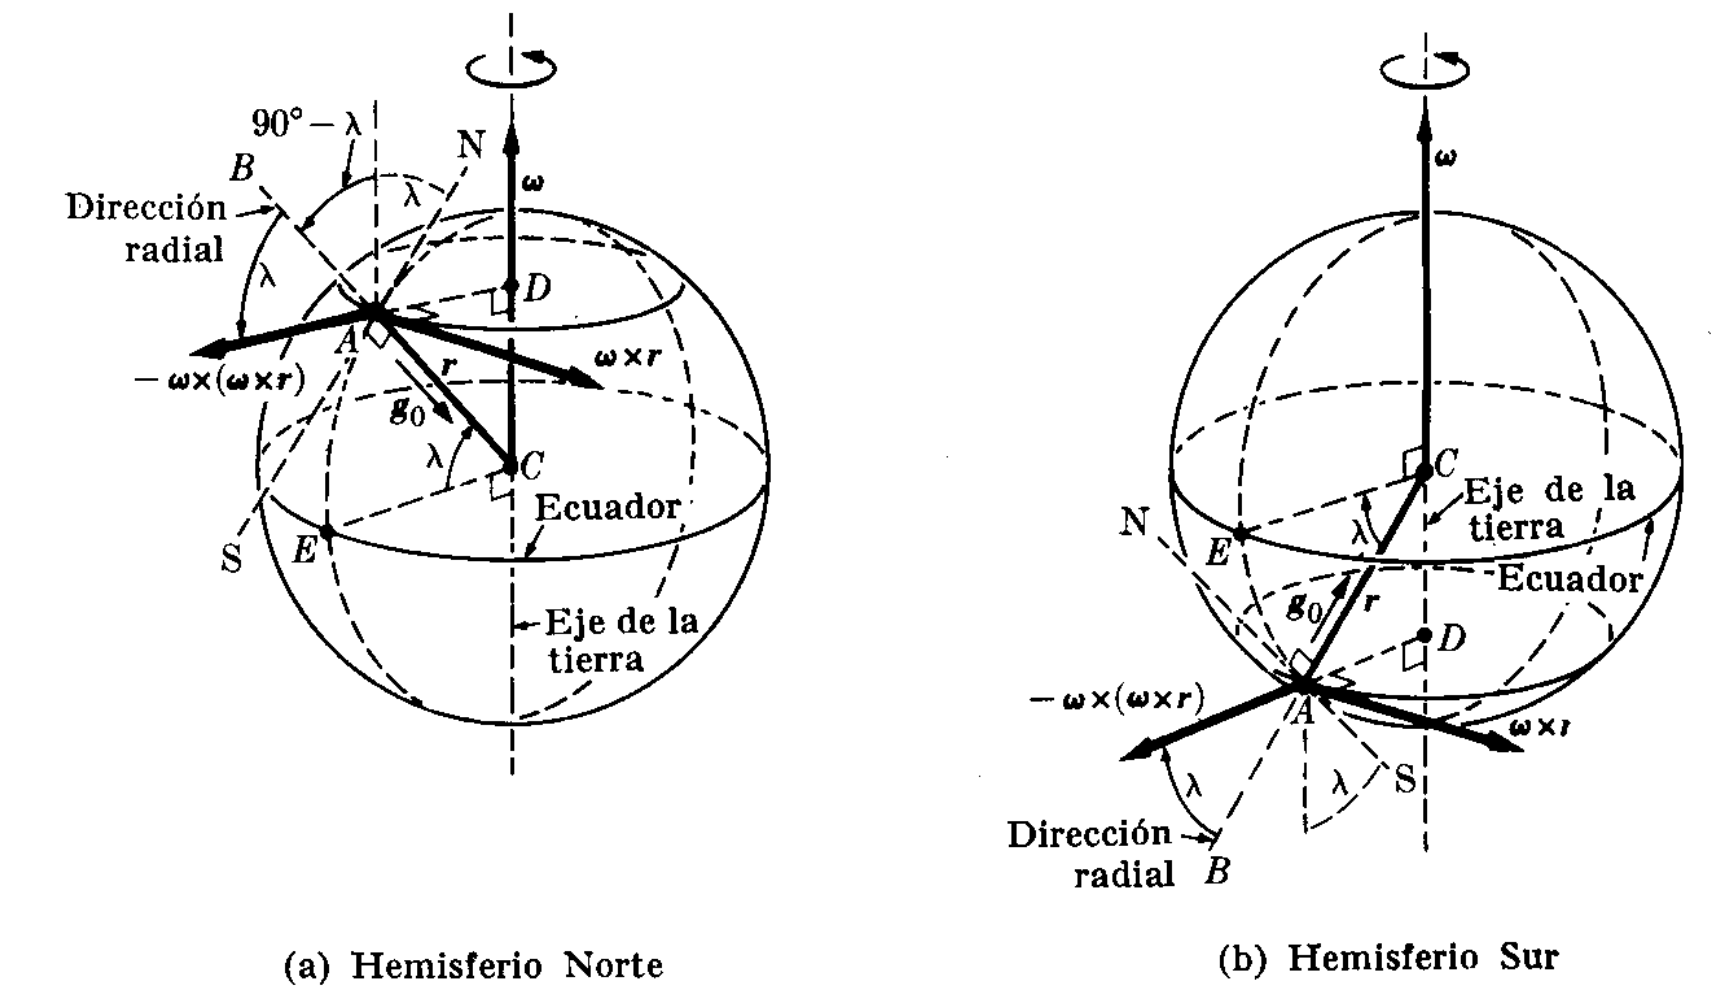
\includegraphics[width=1.05\textwidth]{imagenes/imagenes11/T11IM01.png}
\end{figure}

Vamos a centrarnos en la aceleración efectiva de la gravedad.

\begin{multicols}{2}
Fijándonos en la figura, $\vec g$ apuntará hacia el el sur del $C$, no hacia el centro de la tierra.

Hay que diferenciar entre la \emph{vertical del lugar}, definida por la plomada, y la dirección hacia en centro de la Tierra. En el hemisferio norte, la vertical del lugar pasa por un punto situado al sur del centro de la Tierra, $C$. 
\begin{figure}[H]
	\centering
	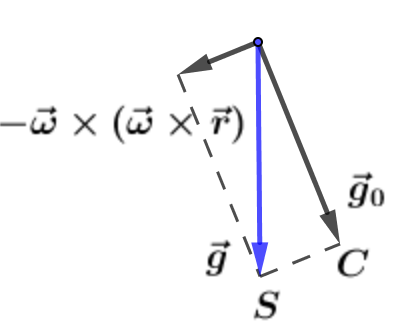
\includegraphics[width=.45\textwidth]{imagenes/imagenes11/T11IM02.png}
\end{figure}
\end{multicols}

La siguiente figura muestra la desviación de la dirección de un cuerpo que cae debido a la aceleración centrífuga:hacia el sur en el hemisferio norte y hacia el norte en el hemisferio sur.

\begin{figure}[H]
	\centering
	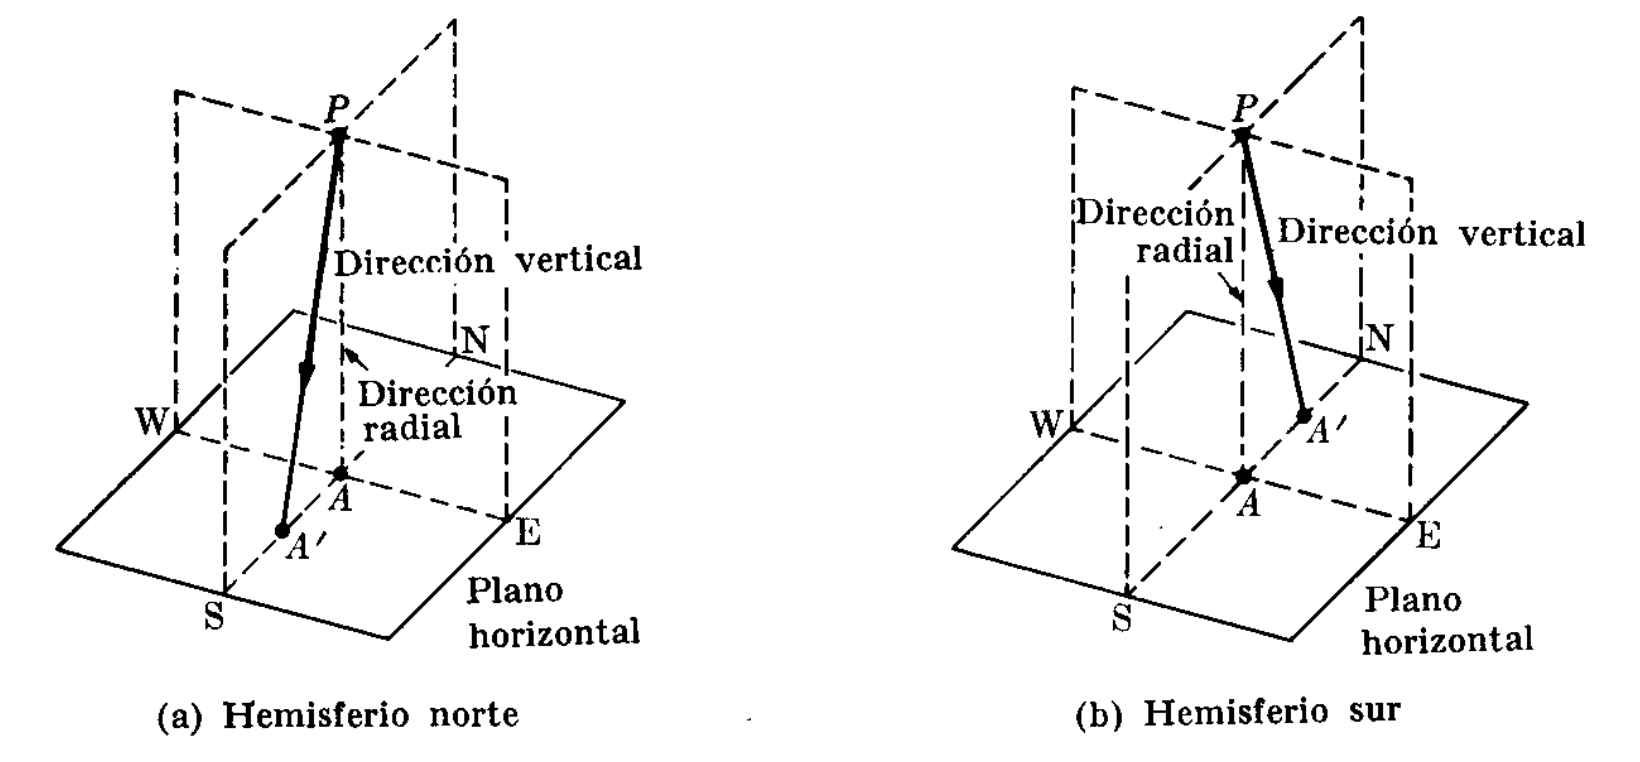
\includegraphics[width=1\textwidth]{imagenes/imagenes11/T11IM08.png}
\end{figure}


$\vec \omega \times (\vec \omega \times \vec r)= \omega \cdot \omega \cdot r \cdot \cos \lambda =\omega^2 \ r \ \cos \lambda$

Vamos a descomponer la aceleración centrífuga, $\vec \omega \times (\vec \omega \times \vec r)$, en dos componentes, según la horizontal de lugar $NS$ y según la dirección radial $AC$

$|\vec \omega \times (\vec \omega \times \vec r)|=\omega ^2 r \sin(90^o-\lambda)=\omega^2r \cos \lambda$

\begin{figure}[H]
	\centering
	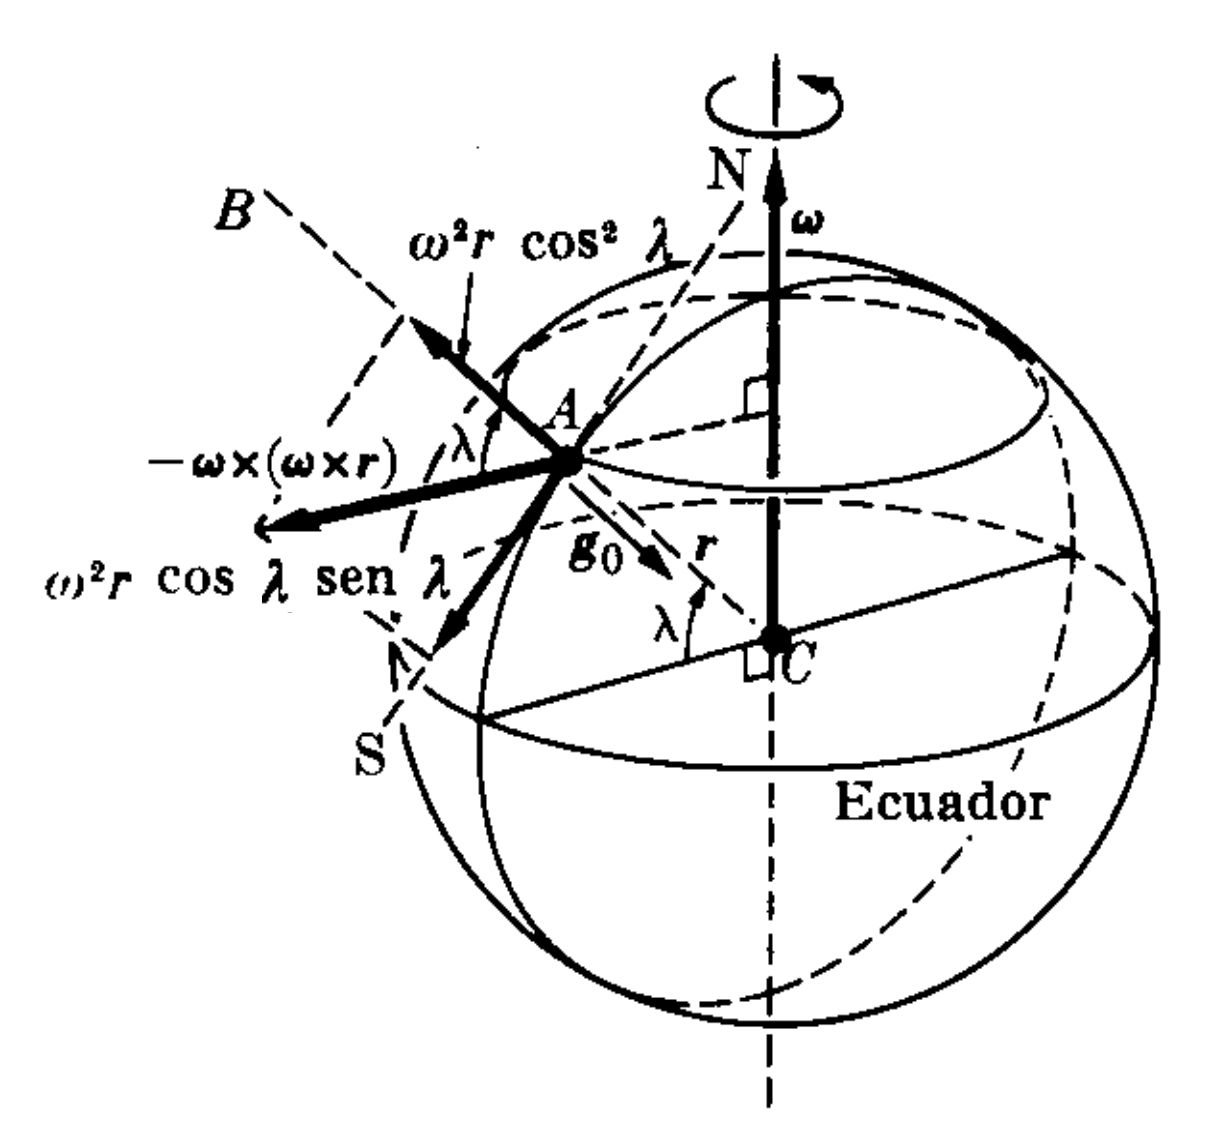
\includegraphics[width=.8\textwidth]{imagenes/imagenes11/T11IM03.png}
\end{figure}

--- Componente en la dirección radial ($BC$): $\ \omega^2 r \cos \lambda \cdot \cos \lambda = \omega^2 r \cos^2 \lambda$

--- Componente Norte Sur ($NS$): $\qquad \qquad \quad \ \ \omega^2 r \cos \lambda \cdot \sin \lambda = \dfrac 1 2 \omega^2 r \sin (2 \lambda)$

Vectorialmente:

$$\subrayado{ \boldsymbol{ \vec g=\vec u_r\ (g_0-\omega^2 r \cos^2 \lambda)+\vec u_{NS}\ \dfrac 1 2 \omega^2 r \sin 2\lambda } }$$

\begin{figure}[H]
	\centering
	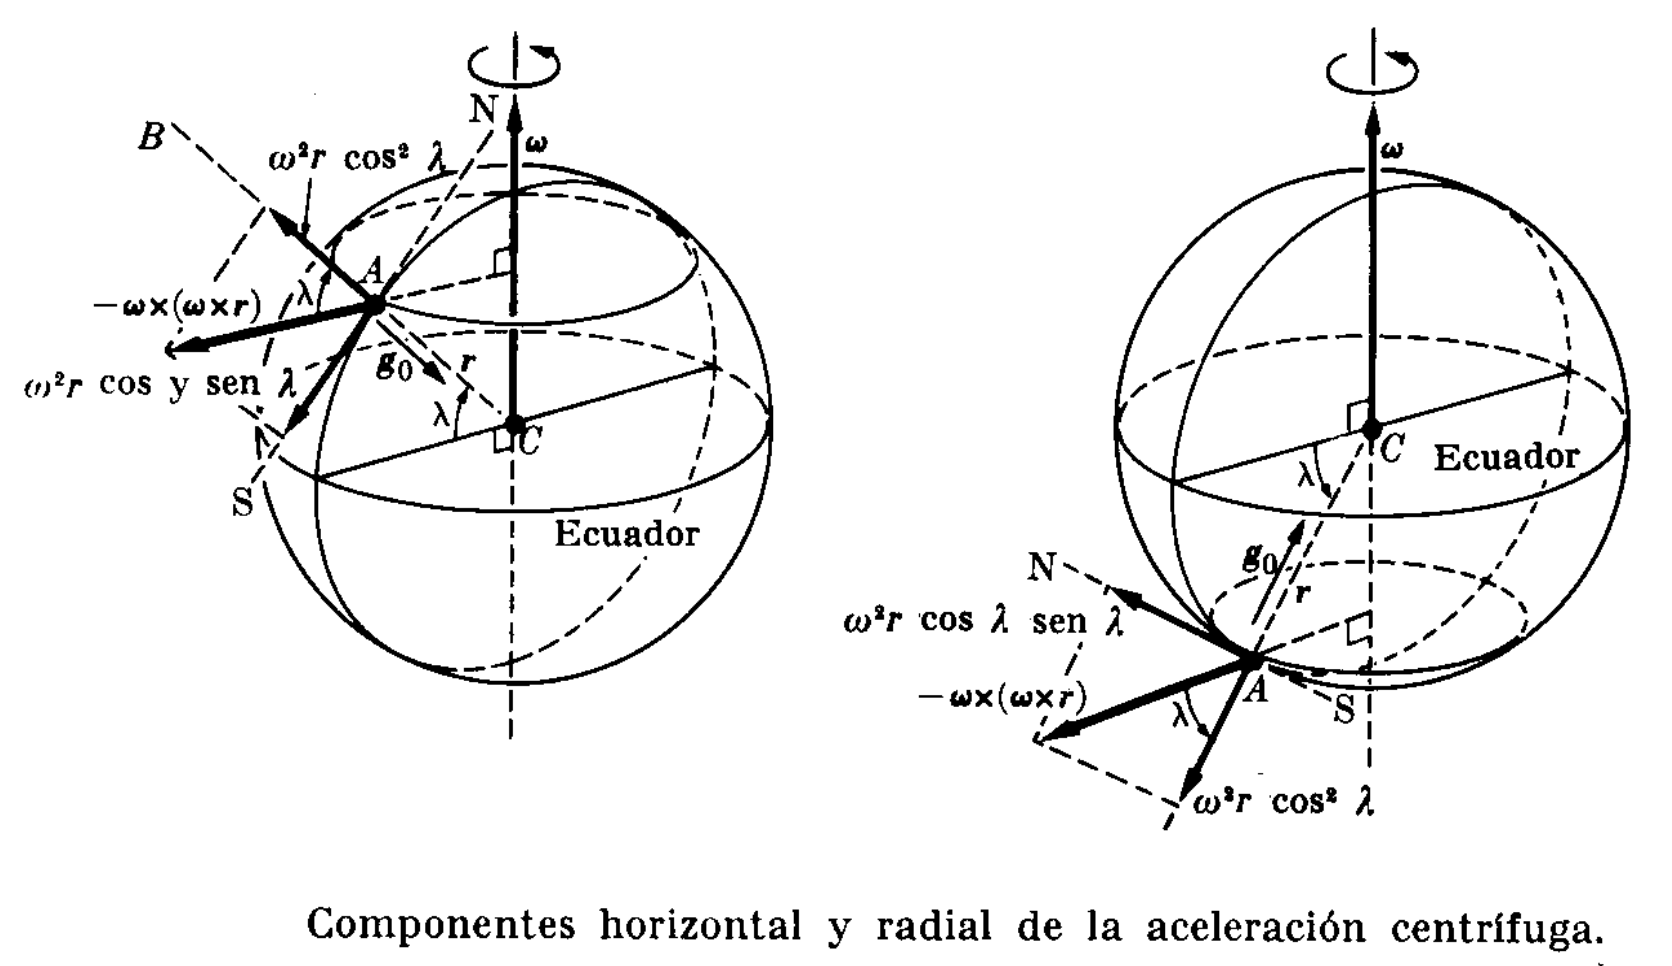
\includegraphics[width=1.05\textwidth]{imagenes/imagenes11/T11IM04.png}
\end{figure}

La aceleración efectiva de la gravedad depende de la latitud $\lambda$ del lugar: $g=g(\lambda)$

La velocidad angular de la Tierra es $\omega=7.292\times 10^{-5} \ \mathrm{rad/s}$. El valor máximo de la componente Norte-Sur de la aceleración efectiva de la gravedad es  $\frac 1 2 \omega^2 r \sim 0.3\%  \text{ de } g_0$, es por esto por lo que, con mucha aproximación, se suele decir que el módulo de $\vec g$ coincide con la componente radial: $\boldsymbol{ g\approx g_0-\omega^2r\cos \lambda }$. $\ g\ $ varía  desde el ecuador a los polos, donde coincide con $g_0$ ya que los polos no giran.

\begin{figure}[H]
	\centering
	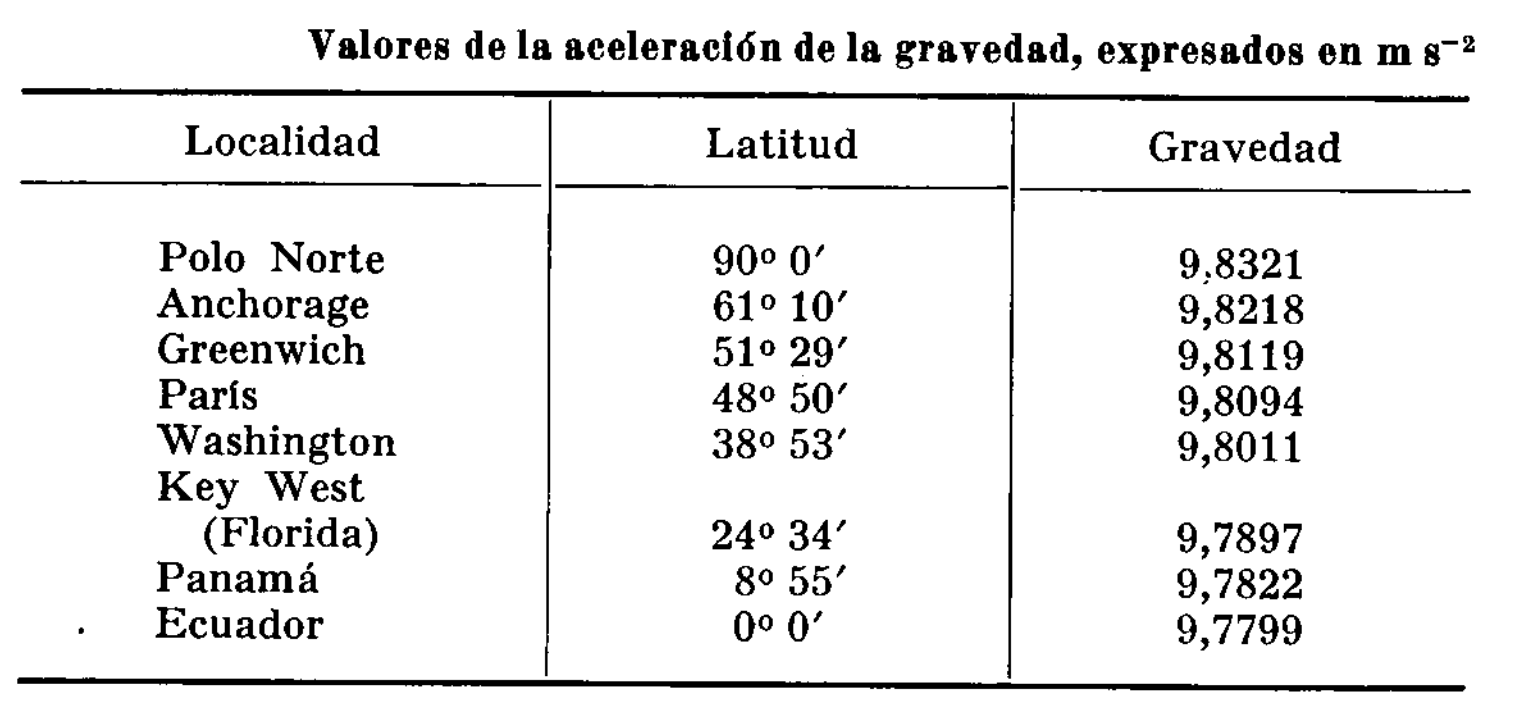
\includegraphics[width=1\textwidth]{imagenes/imagenes11/T11IM07.png}
\end{figure}

En la Tierra hay gran cantidad de agua, fluído, que está en equilibrio cuando adopta forma esférica. La tierra es achatada debido a su propia rotación. El semi-eje mayor mide $6378399 \text{ m}$ y el menor $6356912\text{ m}$. La elipticidad o achatamiento viene medida por el cociente $f=\frac{a-b}{a}=0.003867$ por lo que es prácticamente esférica ($f=0$).

Supongamos el siguiente problema físico real: estamos situados sobre un punto de la superficie de la Tierra y queremos encontrar las ecuaciones de movimiento, para ello vamos a integrar la ecuación
$\ \vec a\ '=g-2\vec \omega \times \vec v\ '$. Recordar que $\vec v\ '$ es la velocidad que tiene el cuerpo en estudio respecto al observador móvil y nos es totalmente desconocida.

$|2\vec \omega \times \vec v\ '| \leqslant 2\omega v\ '=14.585\times 10^{-5}\cdot v\ ' \text{ ms}^{-2}$.  Para velocidades $v\ '$ del orden de $10^3 \text{ ms}^{-1}$, $\ 2\omega v\ ' = 14.6\times 10^{-2} \lesssim  1.5\%$ del valor de $g$. Consideraremos pues este valor despreciable frente a $g$ y siempre que $v ' \leq 10^3 \text{ ms}^{-1}$ tomaremos $a\ '= g - 2mv\ ' \approx g$.

Vamos a valernos de este detalle para resolver la ecuación de movimiento por aproximación, las soluciones que encontremos tendrán validez para un rango de velocidades comprendido entre $0$ y $1000 \text{ ms}^{-1}$.

$\vec a\ ' \approx g = \displaystyle \dv{\vec v_1\ '}{t}$. Hemos puesto $v_1\ '$ en lugar de $v\ '$ para destacar que se trata de una aproximación. 

Llamaremos \emph{dirección radial} a la que desde un punto de la superficie de la Tierra apunta hacia su centro y \emph{dirección vertical} a la de la plomada, definida por $g$, la aceleración efectiva de la gravedad.

\begin{multicols}{2}
$\quad $

$\tan \alpha=\dfrac{\dfrac 1 2 \omega^2 r \sin 2 \lambda}{g_0-\omega^2 r \cos^2\lambda}$

$\tan \alpha \approx \dfrac{\dfrac 1 2 \omega^2 r \sin 2 \lambda}{g_0}$

$\tan \alpha \approx 1.7\times 10^{-3}\ \sin 2 \lambda \ \mathrm{rad}$
\begin{figure}[H]
	\centering
	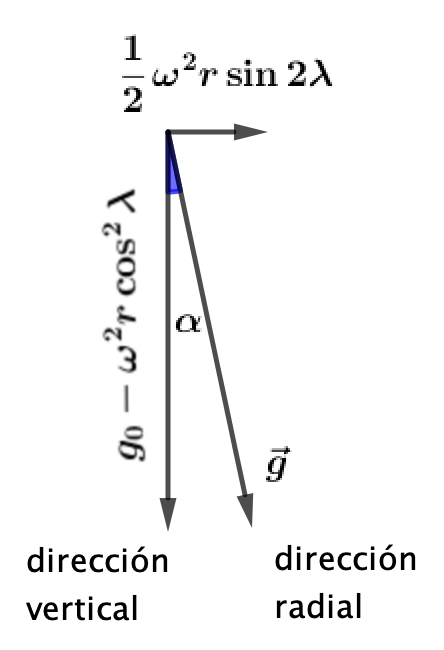
\includegraphics[width=.3\textwidth]{imagenes/imagenes11/T11IM05.png}
\end{figure}
\end{multicols}
\begin{figure}[H]
	\centering
	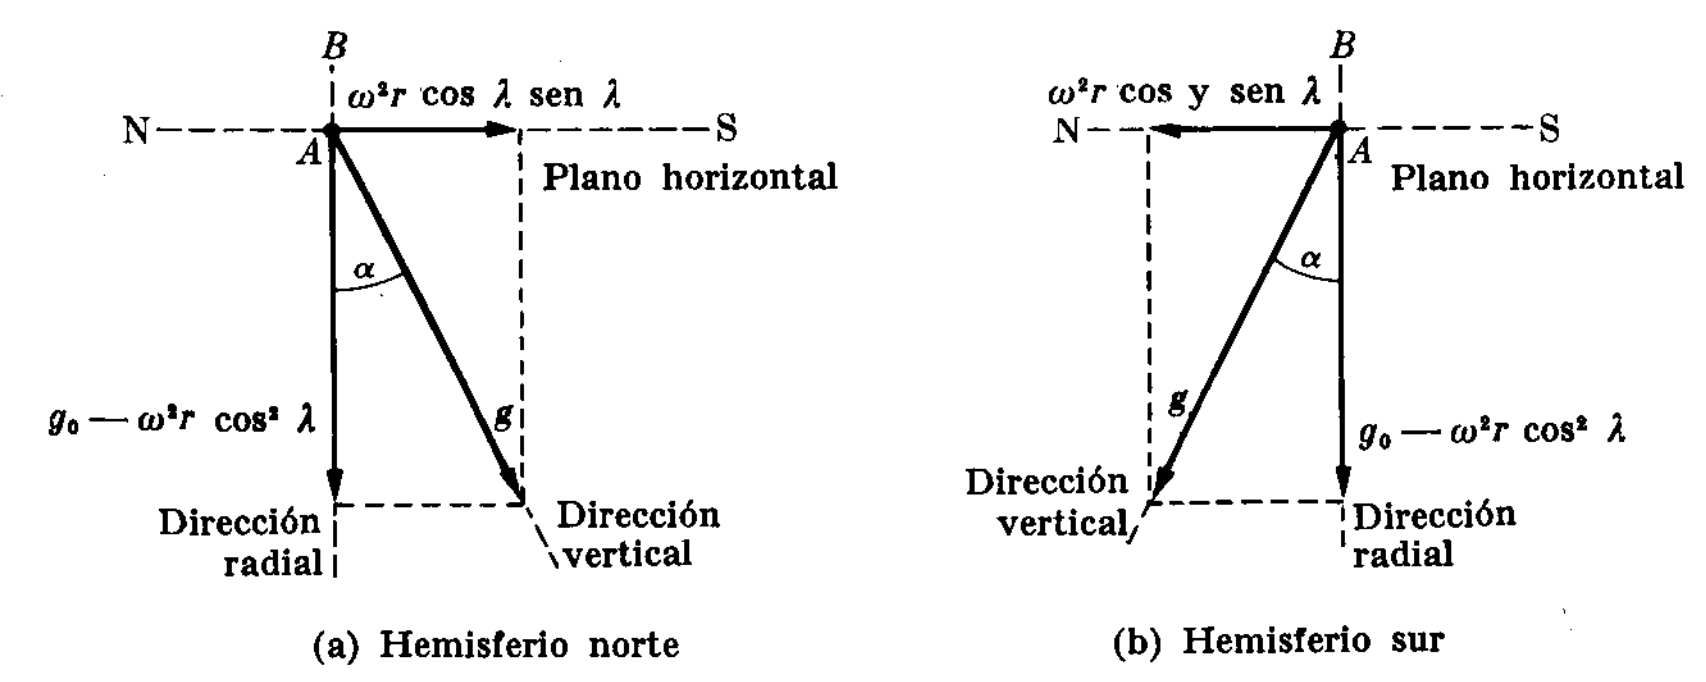
\includegraphics[width=1.05\textwidth]{imagenes/imagenes11/T11IM06.png}
\end{figure}

Lo que indica que $\alpha$ es un ángulo muy pequeño, del orden de un grado, por lo que no cometeremos ningún grave error al considerar, para el rango de velocidades $[0.100] \ \text{ m s}^{-1}$, las direcciones radial y vertical coinciden.


$\vec a'_1=\vec g$, integrando obtendremos la velocidad, que no será $\vec v'_1$ pero será muy similar.

Trabajaremos en el hemisferio norte, el eje $Z$ coincide con el eje de rotación de la Tierra.

$\displaystyle \vec a'_1=\vec g=-g\vec k=\dv{\vec v_i}{t} \to \ \int_{\vec v'_0}^{\vec v'_1}\dd \vec v'_1=-\int_0^t g\vec k ºdd t$
  
$\vec v'_1=\vec v'_0-gt\vec k$, velocidad que no es $\vec v\ '$ pero que no diferirá mucho de ella como hemos dicho.

$\vec a\ '\approx -g\vec k -2\vec \omega \times (\vec v'_0-gt\vec k)= -g\vec k -2\vec \omega \times \vec v'_0+2gt\vec \omega \times \vec k$

$\vec \omega \times \vec k=\omega\cdot 1 \cot \sin (90^o-\lambda)\cdot \ \vec u_{WE}= \omega \cos \lambda \ \vec u_{WE}$ \textcolor{gris}{($WE$ de oeste a este)}

Finalmente:

$$\boldsymbol{ \vec a\ '=-g\ \vec k -2\ \vec \omega \times \vec v_0\ '+ 2\ g\ \omega\ t\ \cos \lambda \ \vec u_{WE} }$$


Teóricamente es todo conocido, $g$ se puede medir con un péndulo, $v_0\ '$ es un dato inicial, $\lambda$ conocido.

Como aplicación veremos dos casos particulares: caída de graves y deriva de proyectiles.

\section{Caída de graves. Desviación hacia el Este.}

Condiciones iniciales (datos): $z'_0=h;\ \vec v'_0=0$. Para $\vec a\ '$ quedan solo dos términos, uno vertical $g$ y otro horizontal $2gt\cos \lambda$:

$\ \vec a\ '=-g\vec k + 2g\omega t\ \vec u_{WE}$

\begin{itemize}
\item Componente horizontal:

$-g=\displaystyle \dv{v_h}{t} \ \to \ \ v_h=-gt=\dv{z'}{t} \ to \ \ z'=h_0-\dfrac 1 2 g t^2\quad$ 

\textcolor{gris}{$v_h$ velocidad vertical, dirección de $h$} 

\item Componente vertical:	

$2g\omega t \cos \lambda =\displaystyle \dv{v_{WE}}{t} \ \to \ \ v_{WE}=g\omega t^2 \cos \lambda =\dv{D_{WE}}{t} \ \to $

$\to \ \ \subrayado{D_{WE}=\dfrac 1 3 g \omega t^3 \cos \lambda } $
\end{itemize}

Como $\cos \lambda > 0 \to $ el desplazamiento es hacia el Este tanto en el hemisferio Norte como en el Sur. 

\section{Lanzamiento de un proyectil. Deriva}

Vamos a elegir un sistema de referencia que nos simplificará el cálculo: $\vec v'_0$ contenido en el plano $Z'Y'$; $\alpha$ es el ángulo de la dirección inicial respecto a la dirección $Y'$; $\varphi$ el ángulo definido por el plano $X'Z'$ y la dirección Norte.

\begin{figure}[H]
	\centering
	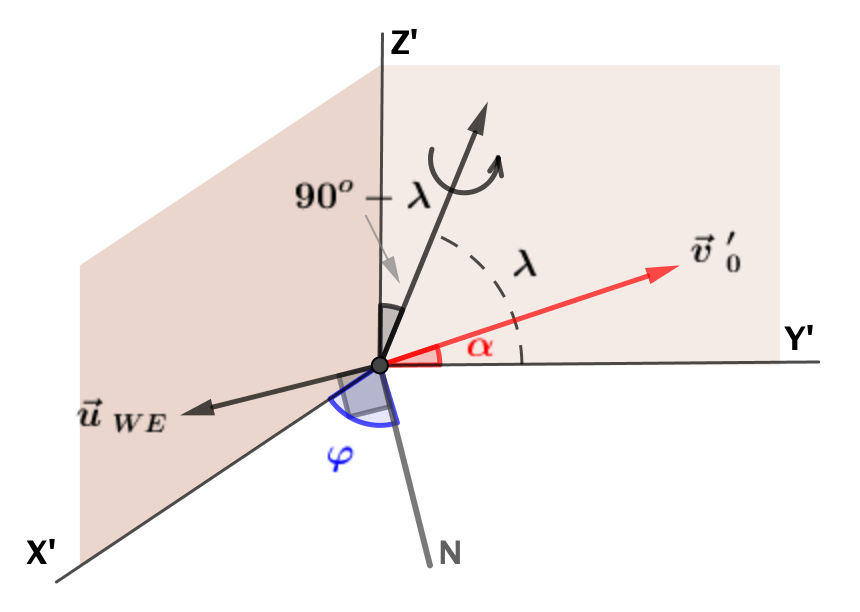
\includegraphics[width=.8\textwidth]{imagenes/imagenes11/T11IM10.png}
\end{figure}

$\vec u_{WE}=\vec i \sin \varphi -\vec j \cos \varphi$

$\vec \omega \times \vec v\ _0'=
\left|\begin{matrix} 
\vec i&\vec j&\vec k \\ \omega_x&\omega_y&\omega_z \\ 0&v\ '_{0y}&v\ '-{0z}
\end{matrix}\right| \leftarrow \
\begin{cases}
\omega_x=\omega \cos \lambda \ \cos \varphi \\
\omega_y=\omega \cos \lambda \ \sin \varphi \\	
\omega_z=\omega \sin \lambda
\end{cases}
\ \textcolor{gris}{\begin{matrix}\cos (90^o-\lambda)=\sin \lambda \\ \sin (90^o-\lambda)=\cos \lambda \end{matrix}}$

Desarrollando se encuentra:

$\vec a\ '=(A_x+B_xt)\vec i+(A_y+B_yt)\vec j+A_z\vec k$

Donde:



$\begin{cases}
\ A_x=2(\omega_z v'_{0y}-\omega_y v'_{0z})=2\omega(v'_{0y}\sin \lambda-v'_{0z} \cos \lambda \sin \lambda	 )\\
\ B_x=2g\omega_y=2g\omega \cos \lambda \sin \varphi
\end{cases}$


$\begin{cases}
\ A_y=2\omega_xv'_{0z}=2v'0z \omega \cos \lambda \cos \varphi\\
\ B_y=-2g\omega_x=-2g\omega \cos \lambda \cos \varphi
\end{cases}$

$\quad \ A_z=-(g+2\omega_x v'_{0y})=-(g+2v'_{0y}\omega \cos \lambda \cos \varphi)$


Vamos, pues, a resolver el problema.

\begin{itemize}
\item Eje X':

$\displaystyle \dv{v'_x}{t}=B_xt+A_x \to \ v'_x=\dfrac 1 2 B_x t^2 + A_x t =\dv{x'}{t} \to$

$\to  \ x'=\dfrac 1 6 B_x t^3+\dfrac 1 2 A_x t^2\quad x'_0=0$
\item Eje Y':

$\displaystyle \dv{v'_y}{t}=B_y t+A_y \to \ v'_y=v'_{0y}+\dfrac 1 2 B_y t^2 + A_y t =\dv{y'}{t} \to$

$\to  \ y'=\dfrac 1 6 B_y t^3+\dfrac 1 2 A_y t^2 +v'_{0y}t \quad y'_0=0$
\item Eje Z':

$\displaystyle \dv{v'_z}{t}=A_z \to \ v'_z=v'_{oz}+ A_z t =\dv{z'}{t} \to$

$\to  \ z'=\dfrac 1 2 A_z t^2 + v'_{0z}t \quad z'_0=0$

\end{itemize}

Y estas son las ecuaciones del movimiento.

Observamos que hay desplazamiento en el eje $x'$, lo cual significa que el proyectil se ha salido del plano vertical $y'z'$ de lanzamiento.

Hagamos unos cálculos: tiempo de vuelo (desde que se lanza el proyectil hasta que vuelve al plano horizontal, $z'=0$).

$z'=0 =t\left( -\dfrac 1 2 gt + v'_{0z} \right) \to \begin{cases}
 \ t=0  \ \text{ momento del lanzamiento}\\ \  -\dfrac 1 2 gt + v'_{0z} =0 \to t_T=\dfrac{2v'_{0z}}{g}=\dfrac{2v'_0\sin \alpha}{g}
 \end{cases}$

--- Calculemos el movimiento en el eje $y'$:

$\qquad \begin{cases}
\ v'_y=v'_0 \cos \alpha=v'_{0y} \\ \ y'=v'_0 \cos \alpha \cdot t	
\end{cases}$

Si el proyectil es lanzado a unos $1000\ \text{ms}^{-1}$, el tiempo de vuelo es del orden de $t_T=2 \times  1000 / 10 =200 \text{ s}$. En estas condiciones, $\frac 1 2 B_y t^2+ A_y t$ y $\frac 1 6 B_y t^3+\frac 1 2 A_y t^2$ son despreciables y solo queda:

$\qquad \begin{cases}
z'=-\dfrac 1 2 g t^2+v'_{0z}t \\ \ y'=v'_0n\cos \alpha \cdot t	
\end{cases}\ $ 

que coinciden con el movimiento parabólico clásico en el caso de que los ejes no giren.

--- Calculemos el movimiento en el eje $x'$:

En este caso, el desplazamiento recibe el nombre de \textbf{deriva del proyectil.}

Tenemos que el tiempo de vuelo es:  $t_T=\dfrac{2v'_0\sin \alpha}{g}$

Sustituimos $A_x$, $B_x$ por su valor en la expresión de $x'$:

$x'=\dfrac 1 6 g\omega t^3 \cos \lambda \sin \lambda + \omega t^2 [\ v\ '_0 \cos \alpha \sin \lambda -v\ '_0 \sin \alpha \cos \lambda \sin \varphi  \ ]$

Si sustituimos $t\to t_T$ obtendremos la expresión para la \emph{deriva horizontal}, lo que se desplaza en $x'$ el proyectil al llegar al suelo:

$x'= \dfrac {4 \omega {v'}_0^3}{g^2} \sin^2 \alpha \  \left[ \ \cos \alpha \sin \lambda-\dfrac 1 3 \sin \alpha \cos \lambda \sin \varphi \ \right]$

Deriva en el hemisferio Norte a una latitud $\lambda$

$\begin{cases}
\ \text{ si } x'>0 \to \text{ la deriva es hacia la derecha} \\	
\ \text{ si } x'<0 \to \text{ la deriva es hacia la izquierda}
\end{cases}$

Debido al signo menos que aparece en la ecuación, hay un ángulo crítico $\alpha_0$ que anula la deriva y el movimiento se restringirá al plano $y'z'$.

$\cos \alpha_0 \sin \lambda = \dfrac 1 3 \sin \alpha_0 \cos \lambda \sin \varphi \ \to \ \ 
 \sin \lambda = \dfrac 1 3 \tan \alpha_0 \cos \lambda \sin \varphi$
 
 $$ \tan \alpha_0=3\ \dfrac {\tan \lambda}{\sin \varphi};\qquad \alpha_0: \text{ ángulo crítico}$$


En el hemisferio Norte, 

$\begin{cases}
\ 0^o\leq \lambda \leq 90^o \to \ \lambda>0 
\\ \ \tan \alpha_0>0 \ \to \ \ 0^o\leq \alpha_0 \leq 90^o
\end{cases}$
En consecuencia, $\sin \varphi>0 \ \to$

$\to \ 0^o\leq \varphi \leq 180^o$ Los ángulos críticos que anulan la deriva van de Este a Oeste, pasando por el Norte.

Análogamente, en el hemisferio sur, los ángulos críticos vas de Este a Oeste, pasando por el Sur.

Pongamos unos datos para hacernos una idea del ángulo crítico. 

En el hemisferio Norte y para un tiro en la dirección Norte, $\varphi = 90^o$ ($y'$ coincide con la dirección Norte), los ángulos para los cuales no hay deriva son:

\begin{table}[H]
\centering
\begin{tabular}{|c|c|c|c|c|c|c|c|c|}
\hline
\textbf{$\boldsymbol{\lambda\ (^o)}$} & 10    & 20    & 30 & 45    & 60    & 70   & 80    & * \\ \hline
\textbf{$\boldsymbol{\alpha\ (^o)}$}  & 27.87 & 47.51 & 60 & 71.56 & 70.10 & 83.1 & 86.63 & * \\ \hline
\end{tabular}
\end{table}

En el hemisferio Norte:
\begin{itemize}
\item Para $\alpha < \alpha_0 \to \ $ en $\ x':\  $ el término sumando es mayor que el que va restando, por lo que $\ x'>0 \ $, hacia la derecha (en el hemisferio Norte).
\item Para  $\alpha < \alpha_0 \to x'=0$, no hay deriva.
\item Para $\alpha > \alpha_0 \to \ $ en $\ x':\  $ el término sumando es menor que el que va restando, por lo que $\ x'<0 \ $, hacia la izquierda.
\end{itemize}

Lo contrario ocurre en el hemisferio Sur.

En los Polos, donde $\lambda=\pm 90^o$, ocurre que $x'>0$ en el Polo Norte y $x'<0$ en el Polo Sur, siendo $x'_{max}=\pm \dfrac{4\omega {v'}_0^3}{g^2} \sin^2 \alpha \cos \alpha$.

En la dirección EW, $\varphi$ vale $0^o$ o $180^o$, con lo que $\sin \varphi=0$ y $x'_{max}=\pm \dfrac{4\omega {v'}_0^3}{g^2} \sin^2 \alpha \cos \alpha \sin \lambda$

Vamos con el \emph{alcance}, $A$, espacio recorrido al cabo de un tiempo $t$:

$A=v'_0\ t \ \to \ \ t=\dfrac A{v'_0} \ \Rightarrow \ \ x'_{M}=\omega \dfrac {A^2}{v'_0} \sin \lambda$, 

deriva horizontal en función del alcance. Hacia la derecha en el hemisferio N ($\sin \lambda>0$) y hacia la izquierda en el hemisferio S.

\textbf{Consecuencias del efecto Coriolis}

\begin{figure}[H]
	\centering
	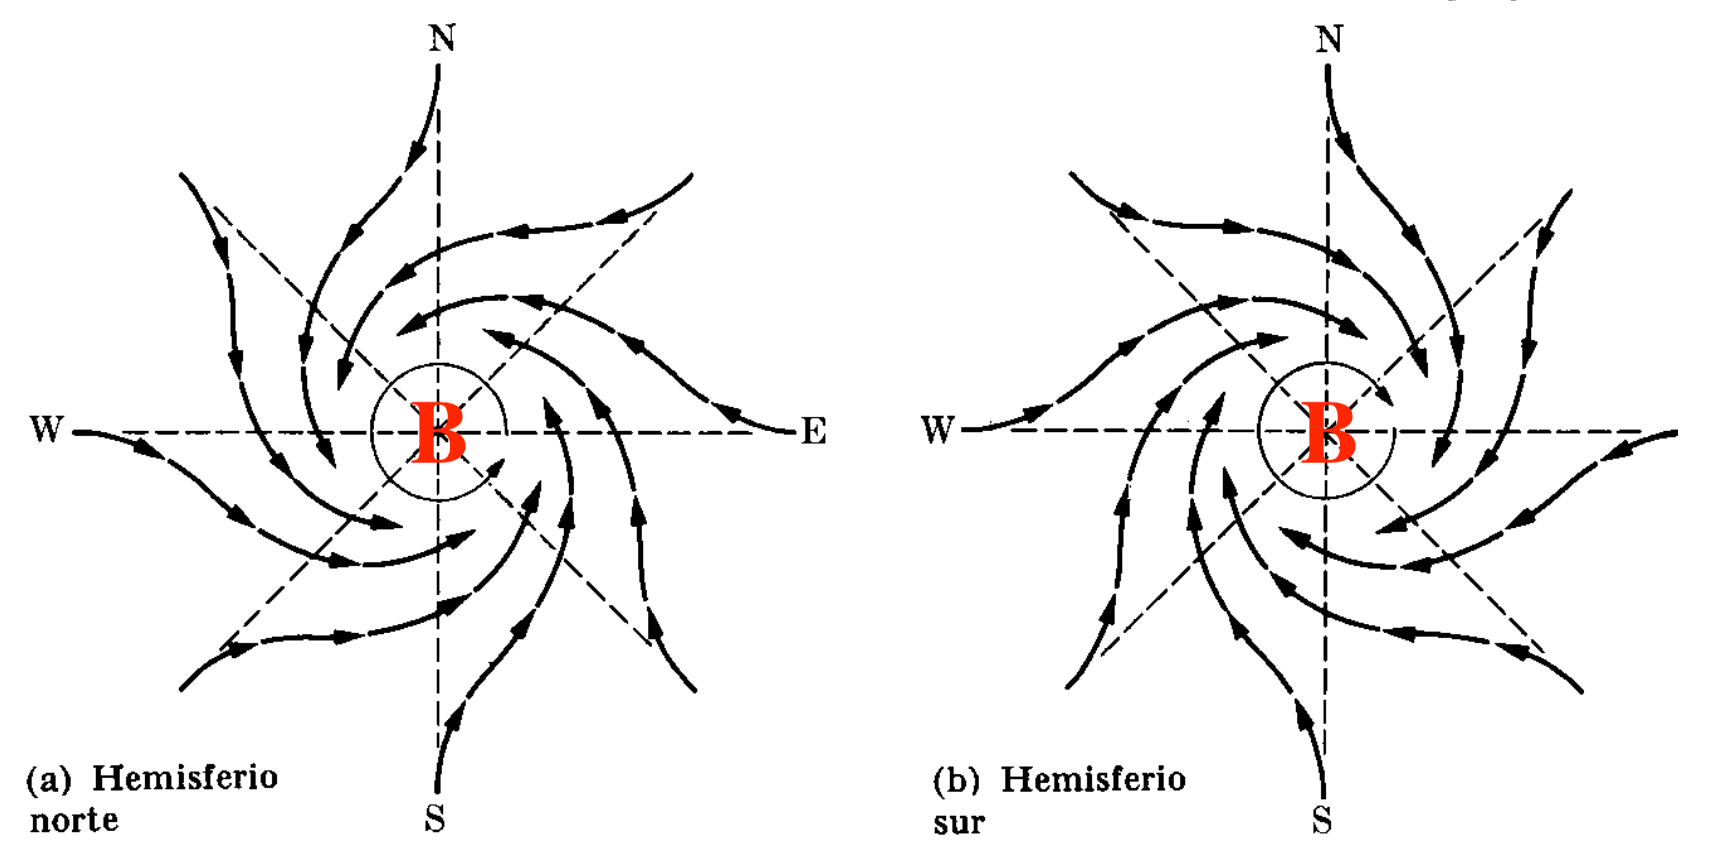
\includegraphics[width=.8\textwidth]{imagenes/imagenes11/T11IM11.png}
\end{figure}

El aire, en las zonas de bajas presiones, gira hacia la izquierda, al contrario de las agujas del reloj. En el hemisferio Sur, las bajas presiones giran en sentido de las agujas del reloj.


El físico francés Bernard León Foucault (1819-1868), en París, construyó un péndulo de $67\ \text{m}$ de largo cuya lenteja era un saco de arena que iba perdiendo un poco de ésta.


En el hemisferio Norte, el plano de oscilación se mueve en dirección a las agujas del reloj. Al contrario en el hemisferio Sur. Se puede demostrar que el ángulo de rotación cada hora es $15^0 \sin \lambda$.

\begin{figure}[H]
	\centering
	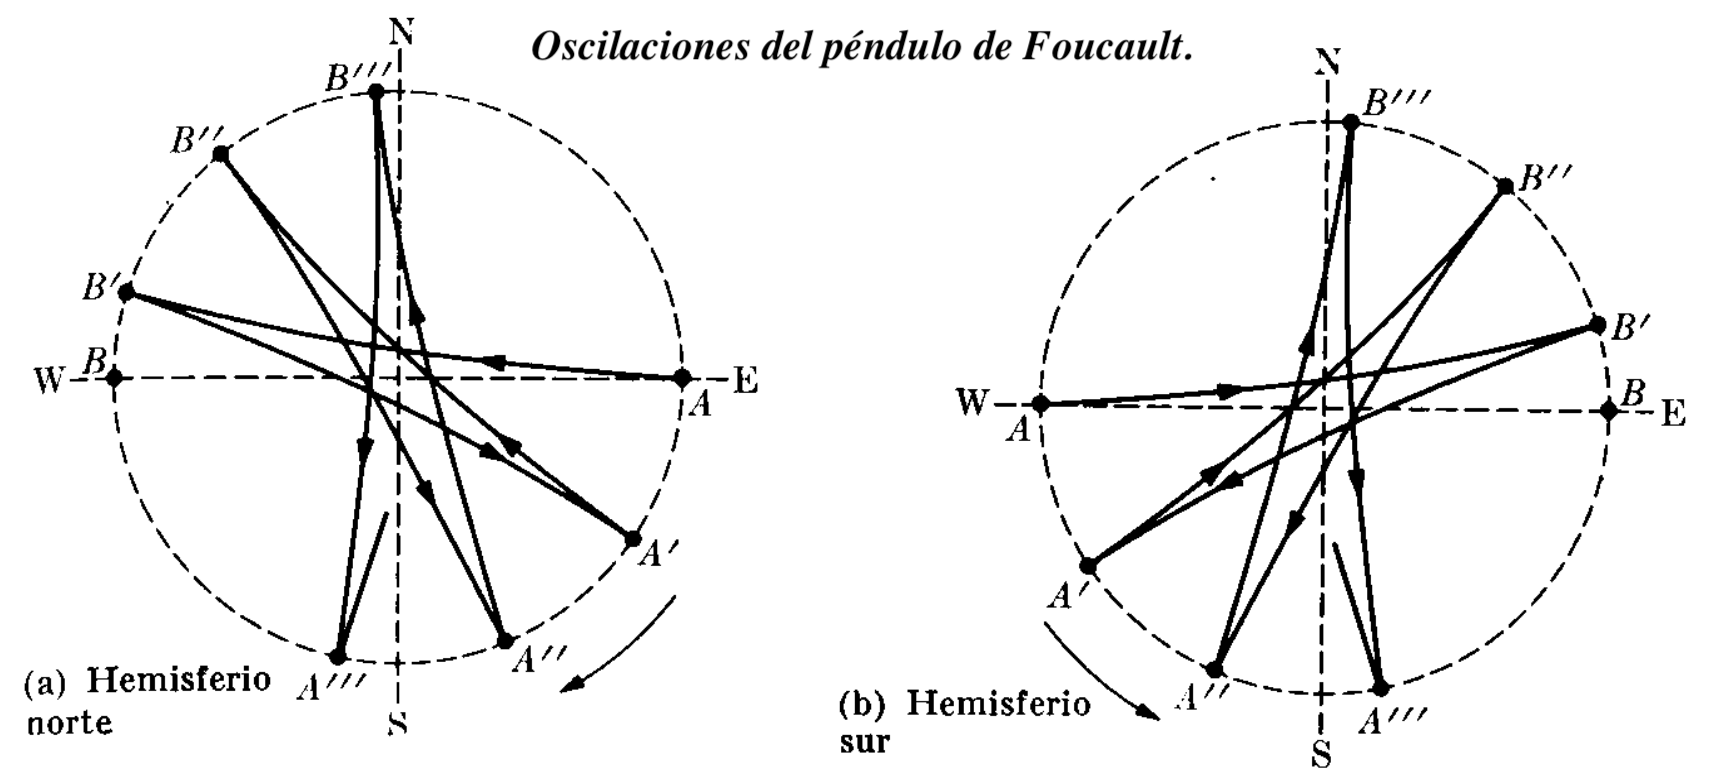
\includegraphics[width=.85\textwidth]{imagenes/imagenes11/T11IM13.png}
\end{figure}

\begin{miparrafo}
Aún si la tierra hubiese estado siempre cubierta de nubes, el experimento del péndulo de Foucault habría demostrado que la Tierra está girando sobre sí misma.	
\end{miparrafo}



\section{Cinemática del sólido rígido}

Un cuerpo \emph{sólido rígido} es aquel cuerpo que está constituido por un sistema de partículas tal que las distancias entre las distintas partículas permanecen inalteradas y constantes en el tiempo.

Sea $x', \ y',\ z'$ un sistema de referencia solidario son el cuerpo. 
\begin{figure}[H]
	\centering
	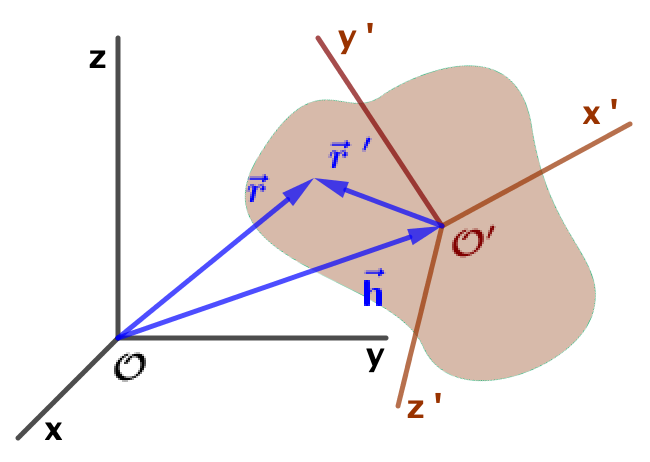
\includegraphics[width=.5\textwidth]{imagenes/imagenes11/T11IM14.png}
\end{figure}

Vimos: $\ \vec v=\vec v\ '+\vec \omega \times \vec r\ '+ \displaystyle \left( \dv{\vec h}{t} \right)_{\mathcal O}$

La velocidad de un punto $P$ del cuerpo respecto de $\mathcal {O}$ es igual a la velocidad respecto de $\mathcal {O'}$ más el producto vectorial de la velocidad angular de la Tierra por el vector de posición del punto $P$ del cuerpo visto desde $\mathcal{O'}$ más la velocidad con que se desplaza $\mathcal{O'}$ respecto de $\mathcal{O}$.

En el sólido rígido, la distancia entre $\mathcal {O'}$ y $P$ no varía, por tanto $\vec v\ '=0$

$\displaystyle \left( \dv{\vec h}{t} \right)_{\mathcal O}=\vec {v'}_0$

Luego: $\ \boldsymbol{ \vec v\ '=\vec {v\ '}_0+\vec \omega \times \	\vec r\ ' }$

\textcolor{gris}{Téngase en cuenta, en problemas, que $\ \vec v\cdot \vec \omega = \vec v\ '_0 \cdot \vec \omega = cte $.}

En el capítulo anterior vimos que:

$\vec a=\vec a\ '+\vec \omega \times (\vec \omega \times \vec r\ ')+ 2 \vec \omega \times \vec r\ '+ \dot{\vec \omega}\times \vec r\ ' + \displaystyle \left( \dv[2]{\vec h}{t} \right)$

Como $v \ ' = 0 \to \vec a\ '=0$, $\quad \displaystyle \left( \dv[2]{\vec h}{t} \right)_{\mathcal {O}}=\vec a_0$, aceleración con la que se desplaza $\mathcal {O'}$ respecto de $\mathcal{O}$.

$\vec a=\vec a_0+\vec \omega \times (\vec \omega \times \vec r \ ' )+ \dot{\vec \omega}\times \vec r\ '$

$\quad$

$\quad$

$\quad$

$\quad$

$\quad$



\begin{figure}[H]
	\centering
	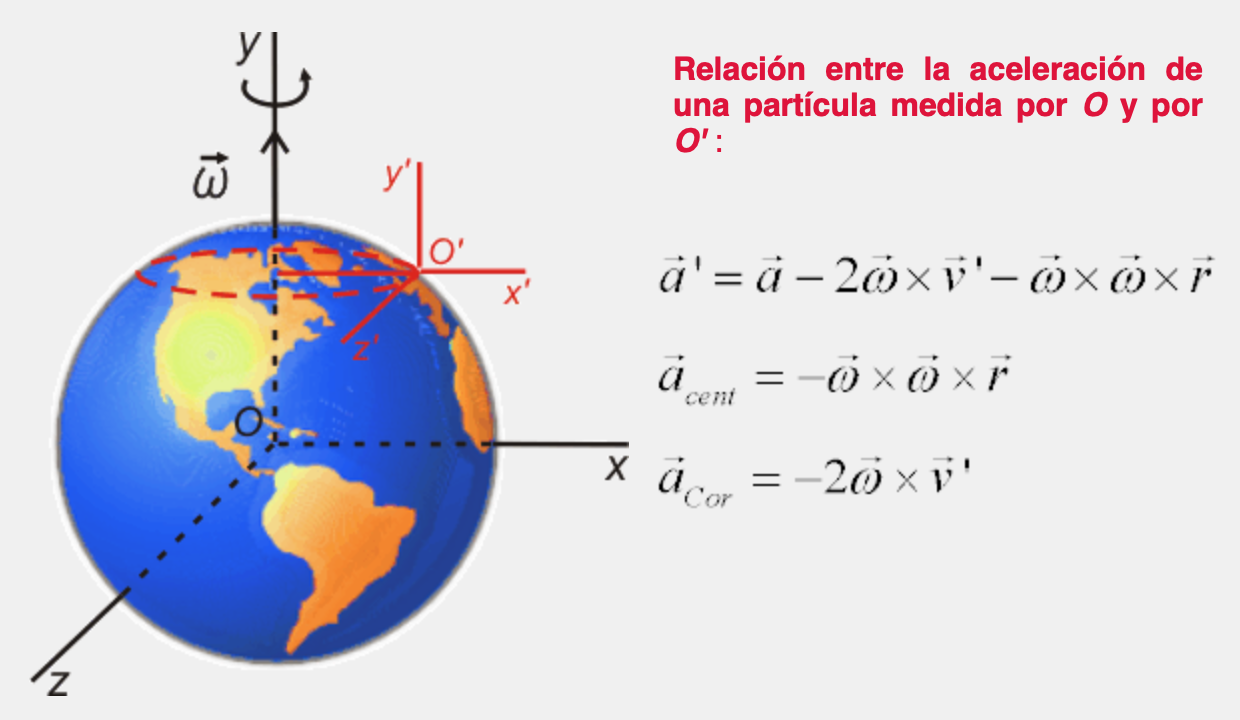
\includegraphics[width=1\textwidth]{imagenes/imagenes10/T10IM10.png}
\end{figure}

$\quad$

$\quad$

$\quad$

$\quad$

\begin{figure}[H]
	\centering
	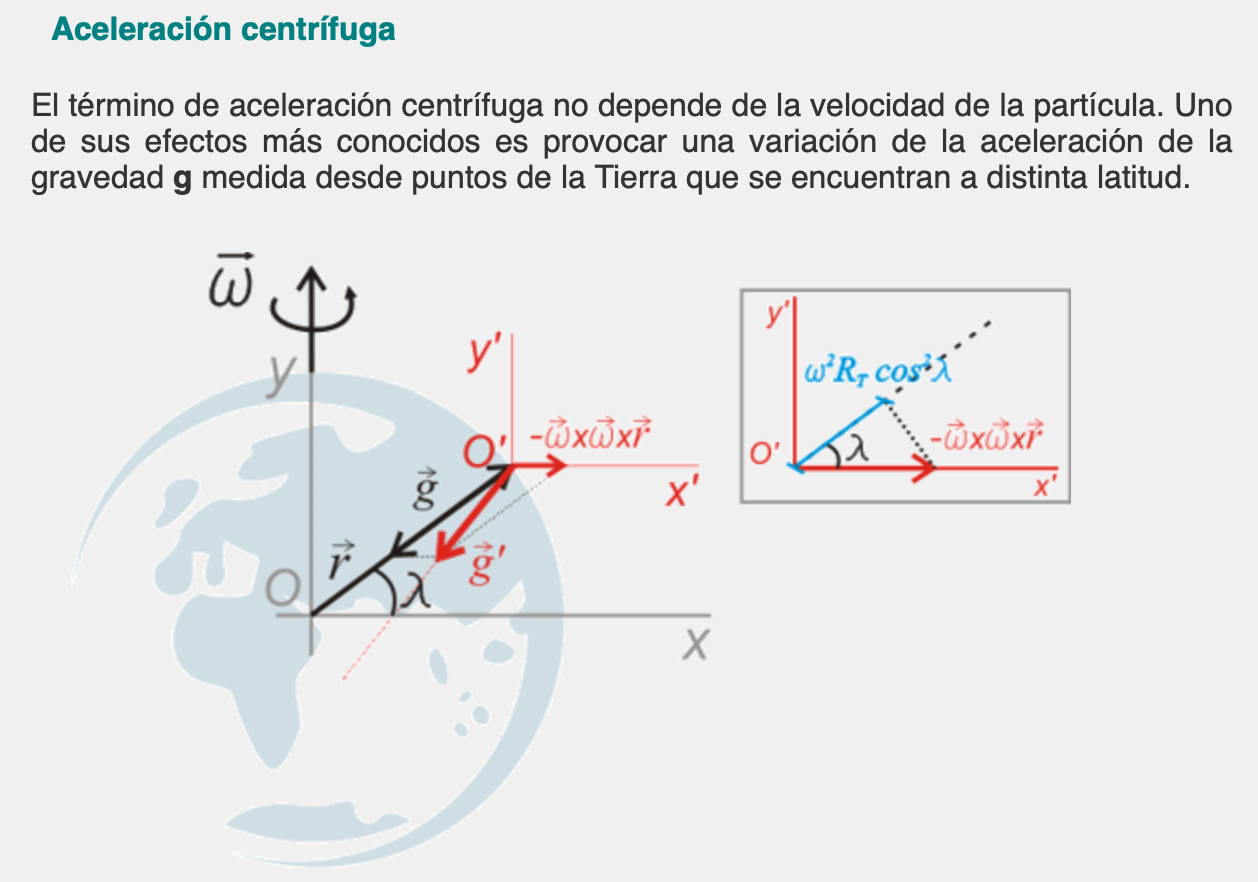
\includegraphics[width=1\textwidth]{imagenes/imagenes10/T10IM11.png}
\end{figure}

\begin{figure}[H]
	\centering
	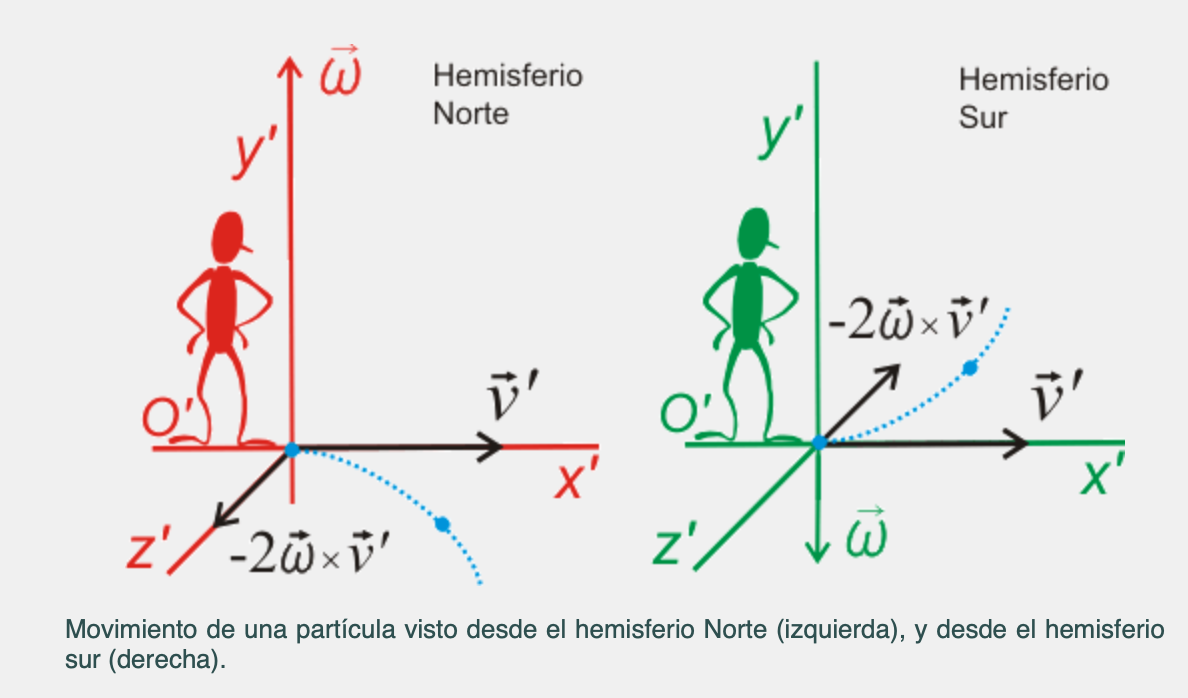
\includegraphics[width=1\textwidth]{imagenes/imagenes10/T10IM12.png}
\end{figure}

$\quad$

\begin{figure}[H]
	\centering
	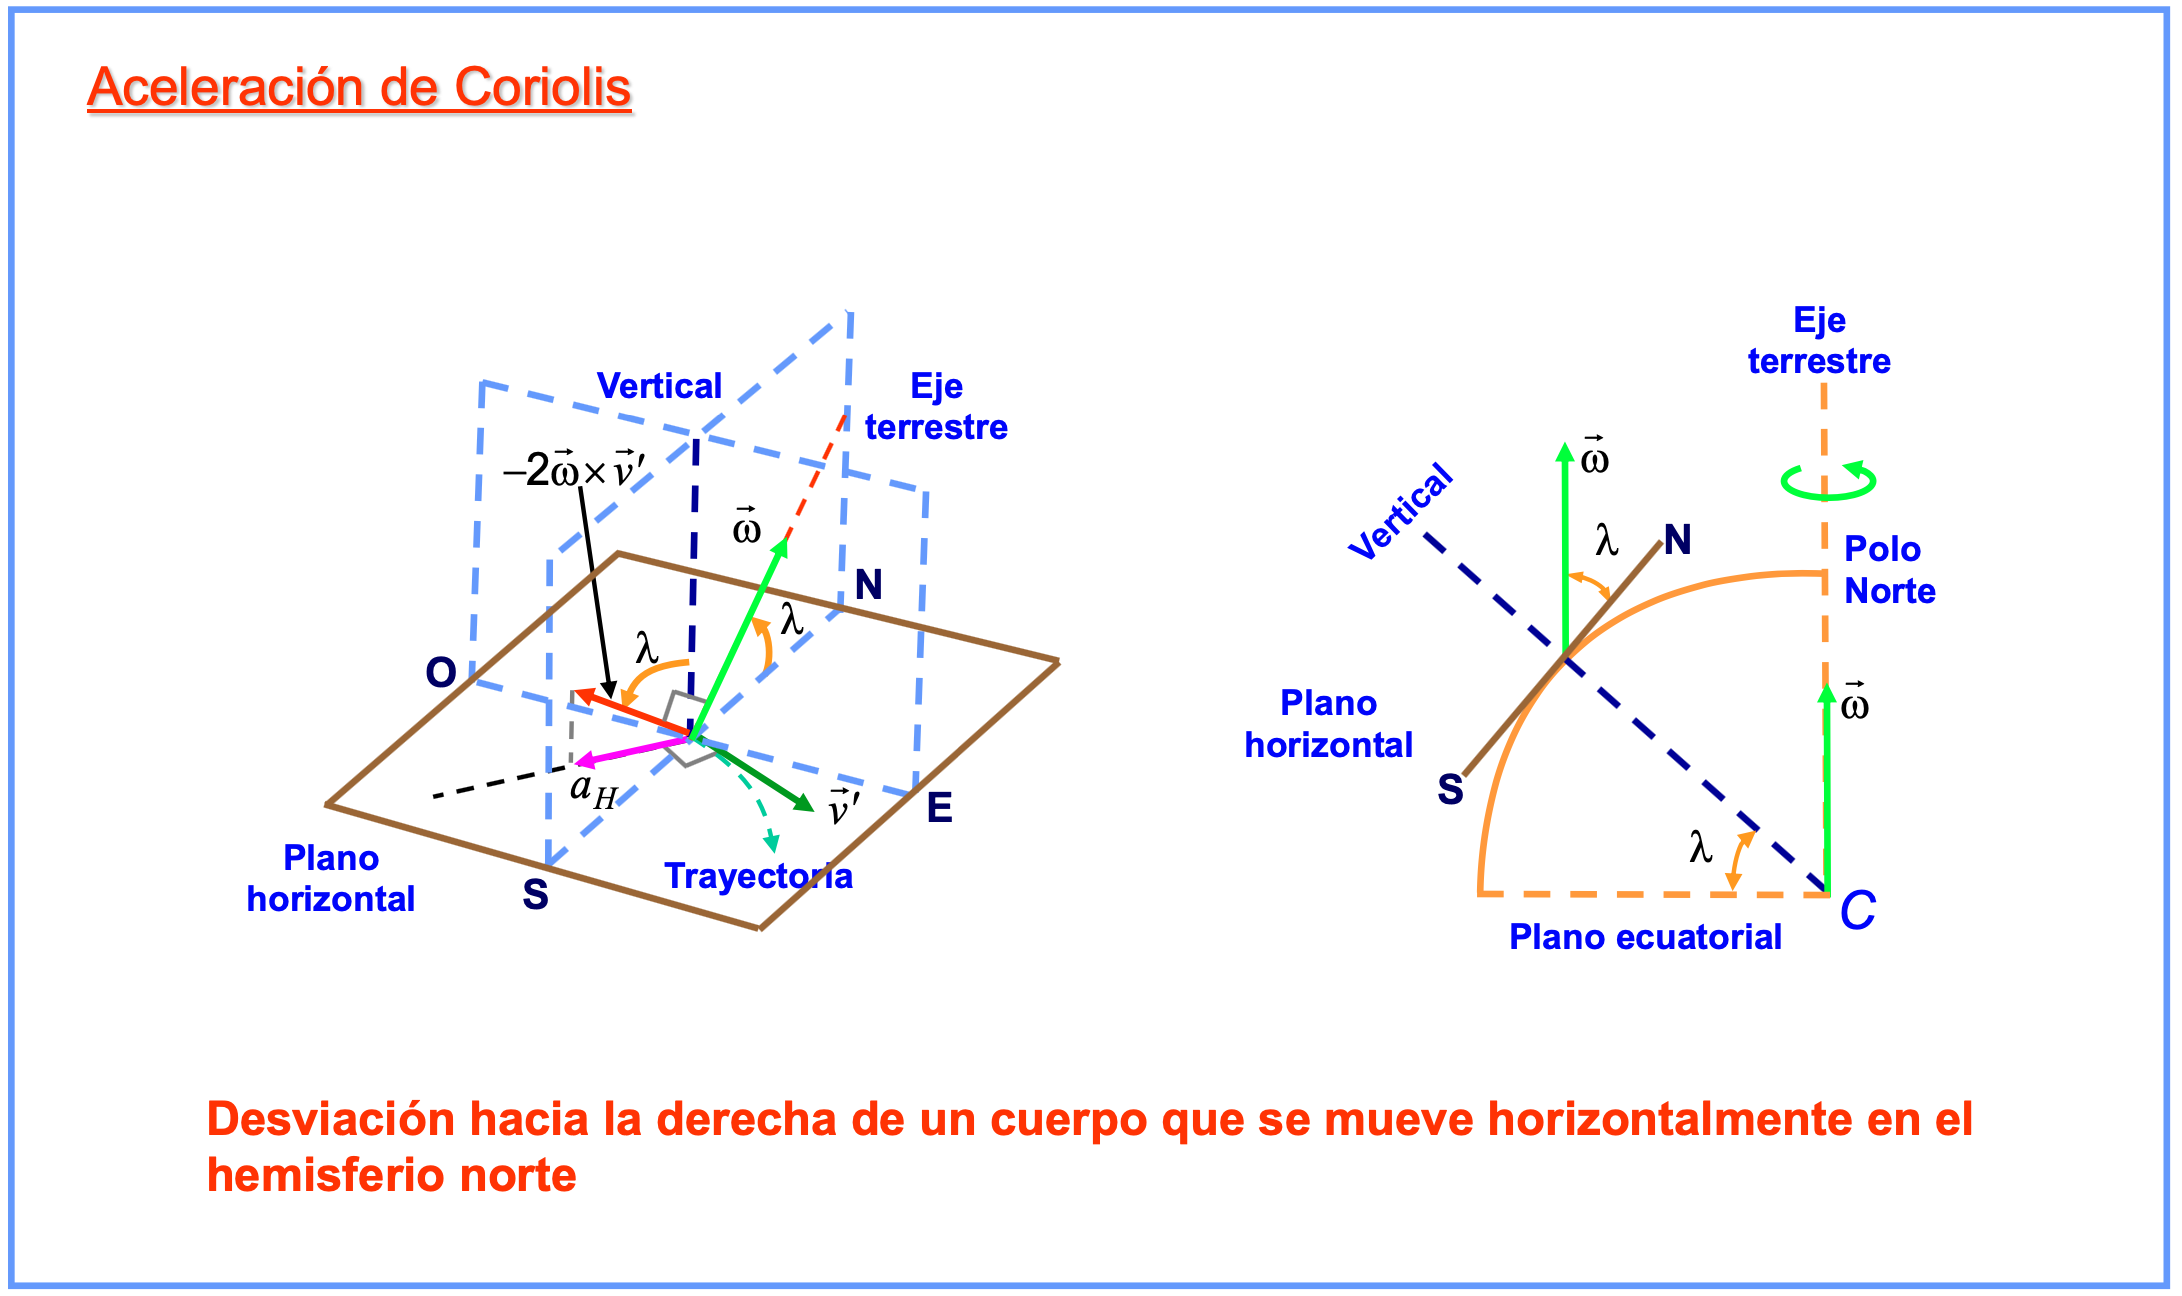
\includegraphics[width=1\textwidth]{imagenes/imagenes10/T10IM13.png}
\end{figure}

$\quad$



\begin{figure}[H]
	\centering
	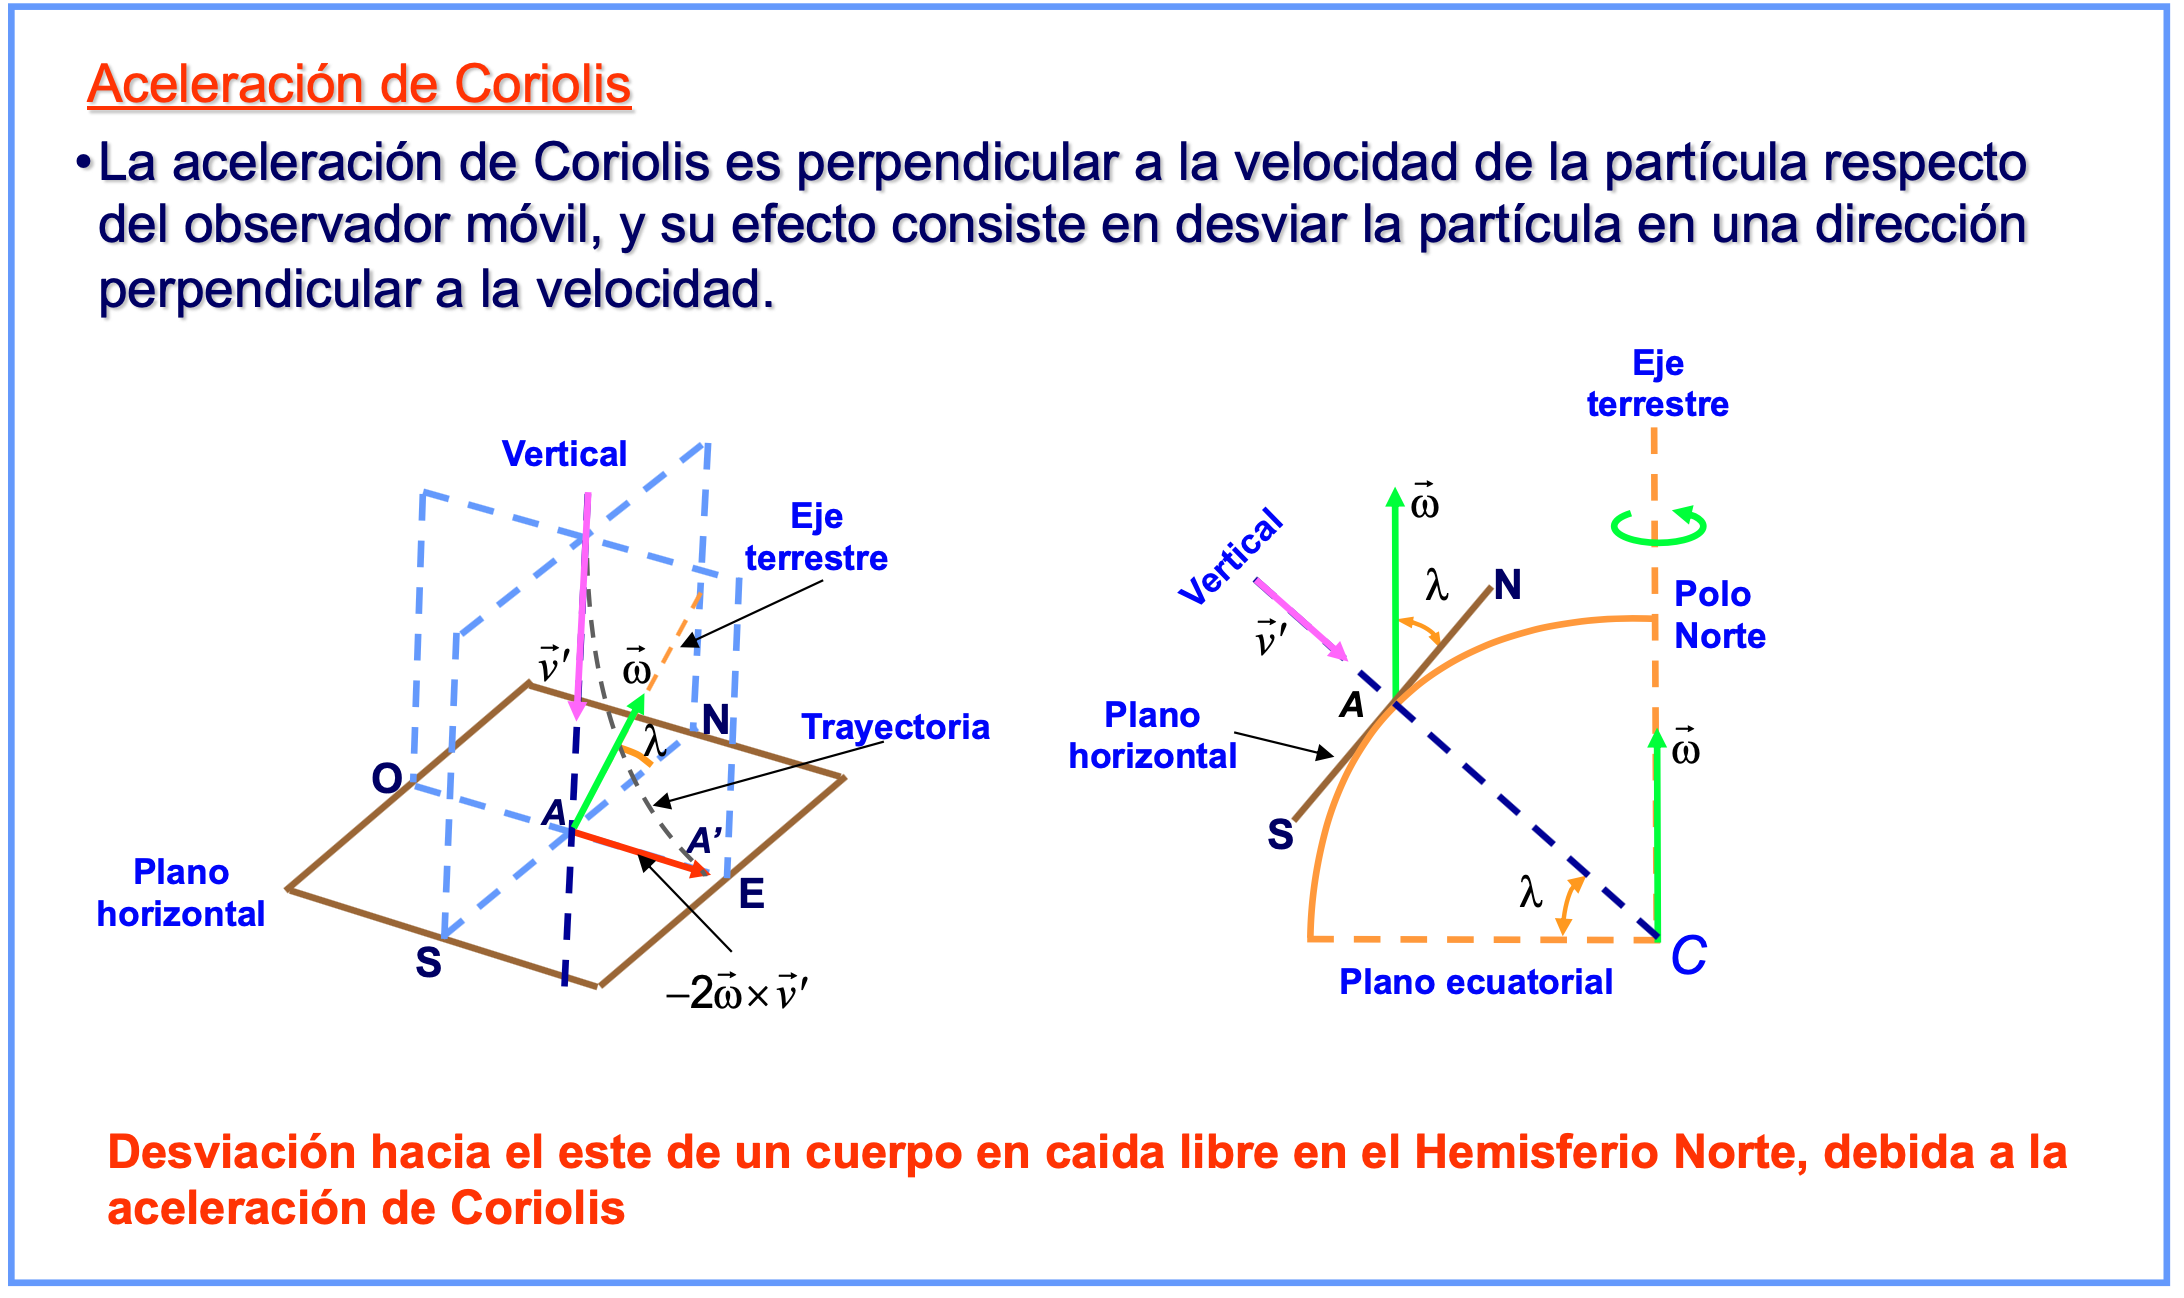
\includegraphics[width=1\textwidth]{imagenes/imagenes10/T10IM14.png}
\end{figure}
$\quad$

\begin{figure}[H]
	\centering
	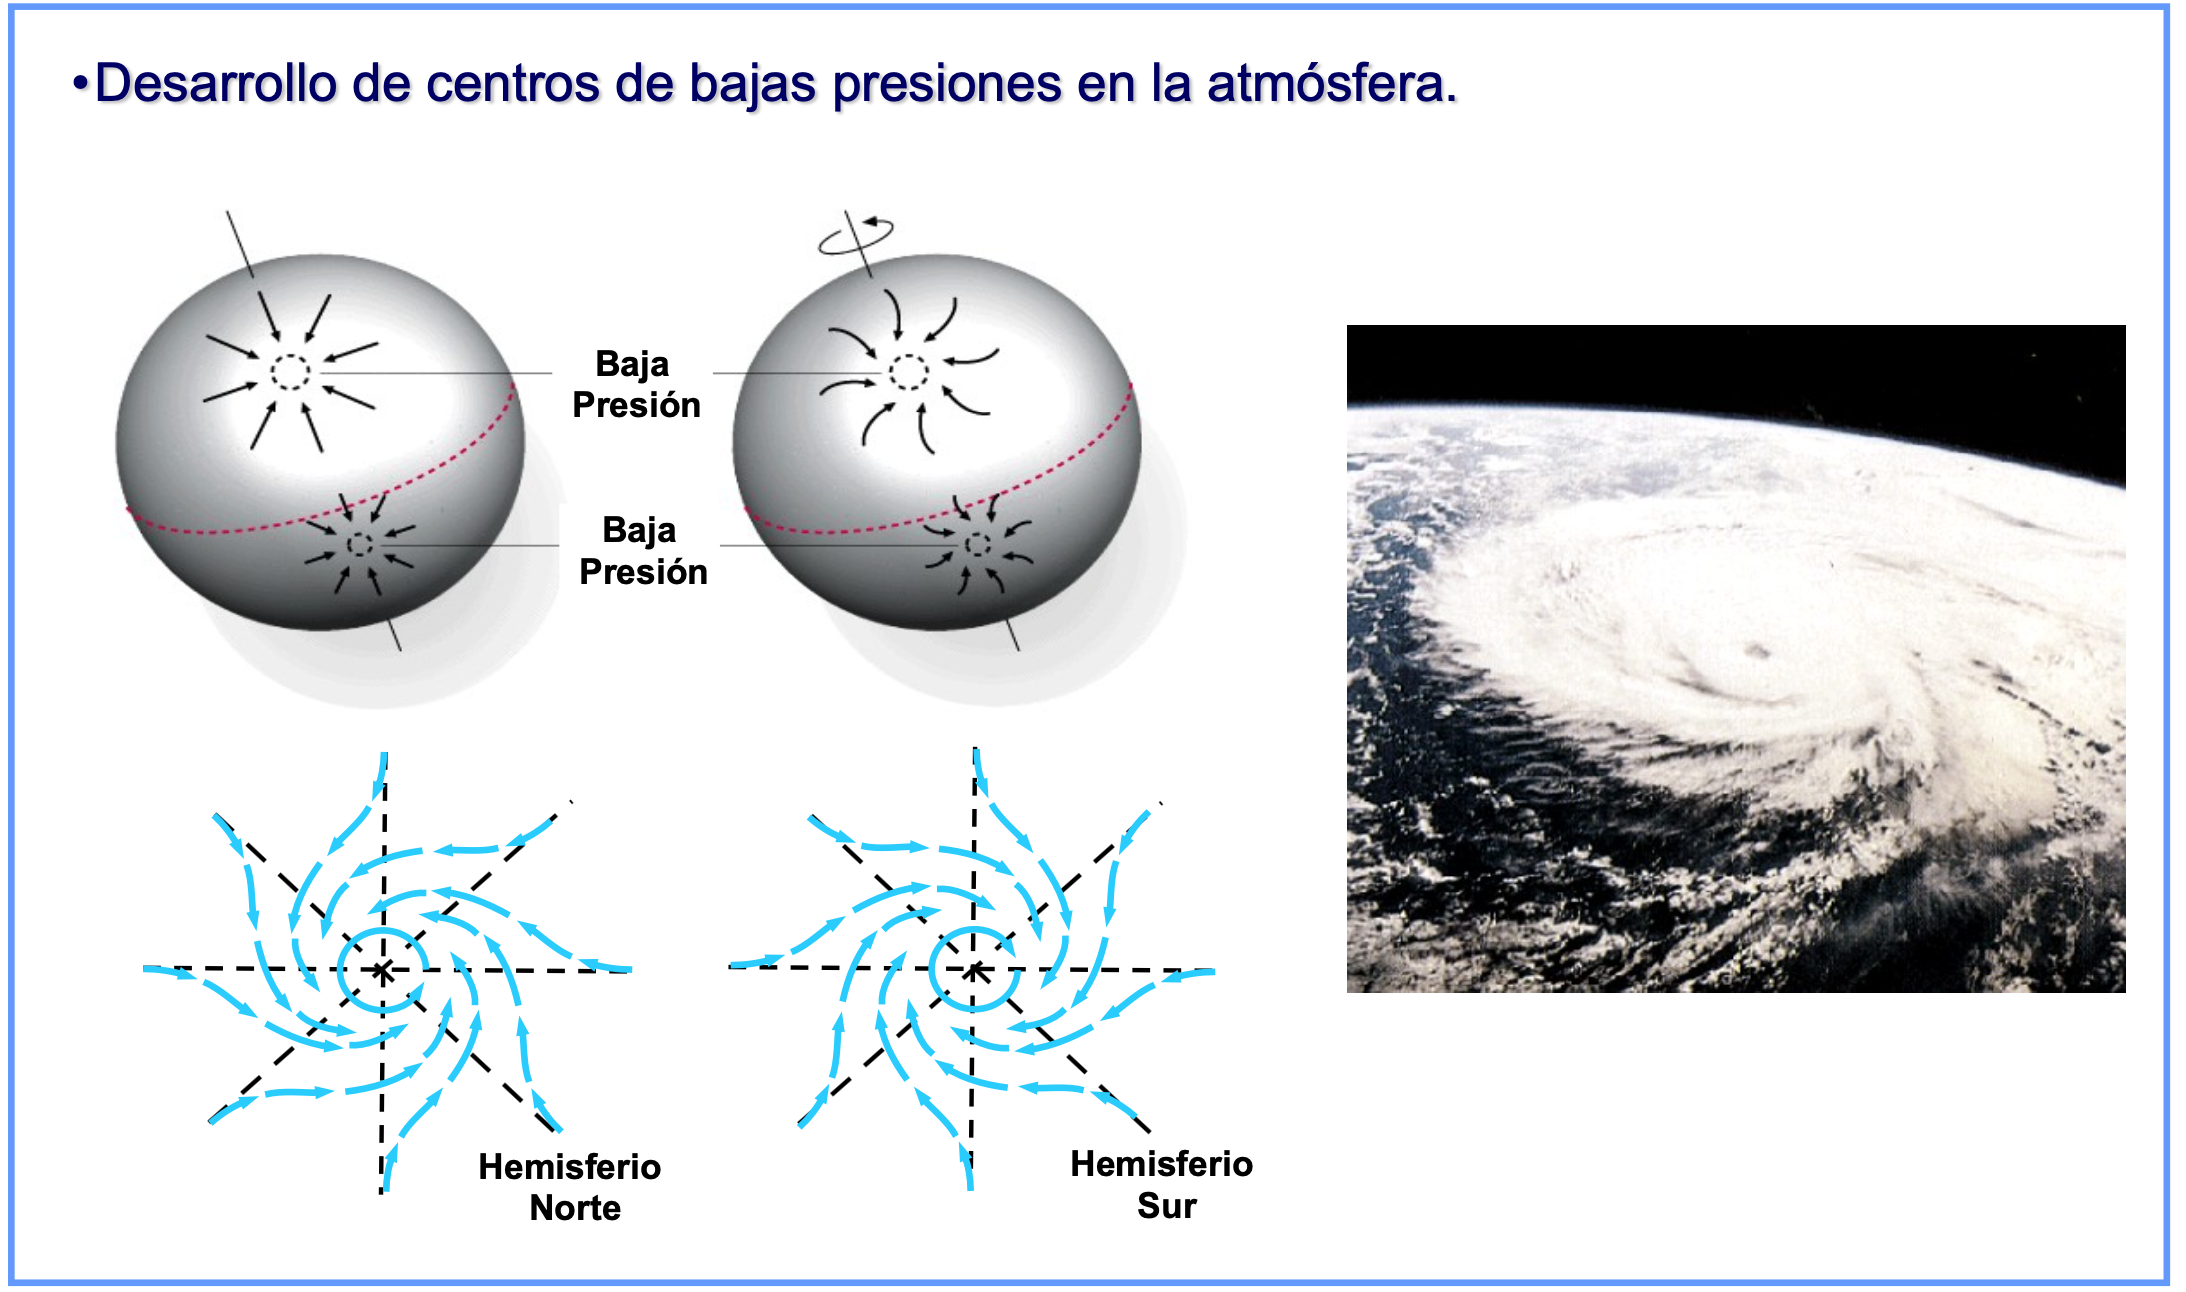
\includegraphics[width=1\textwidth]{imagenes/imagenes10/T10IM15.png}
\end{figure}

\section{Problemas}

\begin{prob}
?`Cuál es la velocidad angular de un punto de la tierra 	respecto a un observador situado en el sol?
\end{prob}

\begin{multicols}{2}
Desde el Sol vemos que un punto $P$ dela tierra da una vuelta a sí misma, $2\pi$ rad, cada día. Al cabo de un año, el ángulo que habrá girado es $300 \times 2\pi$ rad.

$\omega_{TS}=\dfrac{ángulo}{tiempo}=\dfrac{300 \times 2\pi}{365\times 24\times 3600}=7.17\times 10^{-1}\ \text{s}^{-1}$
\begin{figure}[H]
	\centering
	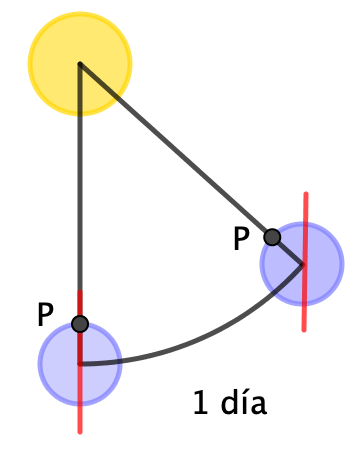
\includegraphics[width=.3\textwidth]{imagenes/imagenes10/T10IM16.png}
\end{figure}
\end{multicols}

\begin{prob}
Una persona embarca en Sidney (Australia) con destino a Oslo (Noruega). Al empezar el viaje en barco, cae enfermo. El barco naufraga y nuestro protagonista despierta en una isla selvática. 

Paseando por la isla se encuentra una emisora de radio. Suponiendo que ha conservado su reloj, ?`Cómo comunicará al mundo civilizado donde se encuentra?	
\end{prob}

Para determinar la \emph{longitud} espera al medio día (cuando el sol proyecta la sombra más corta sobre una estaca que ha clavado en una playa de la isla). Si son las 11, tiene una hora de longitud menos hacia el oeste (el sol sale por el este); si son las 13h, tiene una hora más (hacia el este). Cada hora son $360/24=15^o$


Para determinar la \emph{latitud} a la que se encuentra, coon una liana y una piedra, construye un péndulo de Foucault. Si se desvía hacia la derecha, está en el hemisferio norte; si se desvía hacia la izquierda, está en el hemisferio sur. Además, como el plano de oscilación del péndulo gira $15^o$ por hora, puede determinar su latitud.

\begin{prob}
	Una partícula con una velocidad de $500 \mathrm{m s}^{-1}$ con respecto a la Tierra se dirige hacia el sur a $45^o$ de latitud Norte. Calcular la aceleración centrífuga y de coriolis de dicha partícula
\end{prob}
\begin{multicols}{2}
$r=6.35 \times 10^6 \text{ m}; \omega=7.29 \times 10^{-5} \text{ s}^{-1}; \lambda=45^o; v'=500 \text{ m s}^{-1}$

$a_{centrifuga}=|-\vec \omega \times (\vec \omega \times \vec r)|=\omega^2 r \cos \lambda = 2.39 \text{ m s}^{-1}$

$a_{coriolis}=|2\vec \omega \times \vec v '|=2\omega v' \sin(90^o+\lambda)= $

$=5.55 \times 10^{-5} \text{ m s}^{-1}$
\begin{figure}[H]
	\centering
	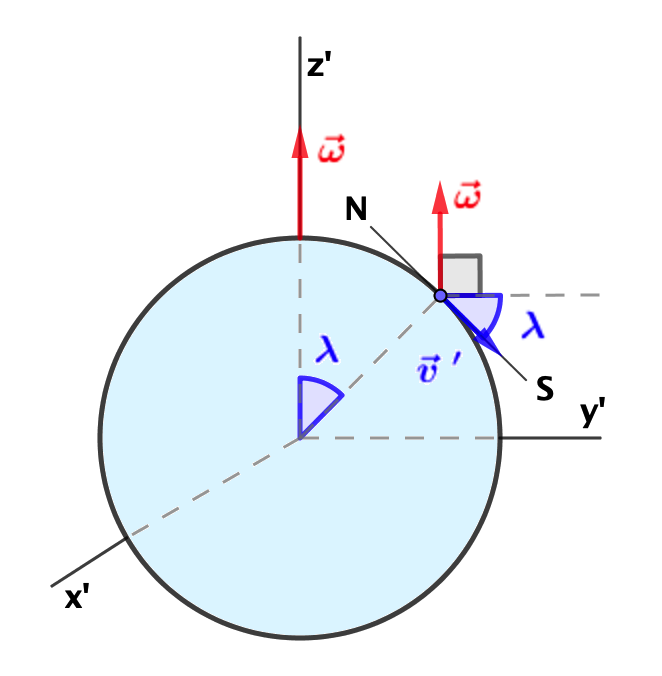
\includegraphics[width=.4\textwidth]{imagenes/imagenes11/T11IM15.png}
\end{figure}	
\end{multicols}


\begin{prob}
Un cuerpo cae desde una altura de $200\ \mathrm{m}$ en un punto de latitud $39^o$	norte. Encontrar la deriva hacia el este con respecto a un punto situado directamente debajo del punto de partida.
\end{prob}

$D_{WE}=\dfrac 1 3 g \omega t^3 \cos \lambda$

$\lambda=39^o; g=9.8\ \text{ms}^{-2}; \ h=200\ \text{m}; \ \omega=7.29\times 10^{-5}\ \text{s}^{-1}$

$h=\dfrac 1 2 g t^2 \to \ t=\sqrt{\dfrac{2h}g}=6.39\ \text{s}$

Sustituyendo, $\ D_{WE}=0.0483\ \text{m}=48.3\ \text{mm}$

\begin{prob}
Desde un punto de la tierra situado a una latitud de $5^o$ N, se dispara un proyectil con velocidad inicial de $800\ \mathrm{m s}^{-1}$ en dirección NW.
\vspace{-3mm} %************************************
\begin{changemargin}{5mm}{5mm} 
	a) Determinar el ángulo crítico de elevación del disparo para que el proyectil no sufra deriva.

	b) Si el ángulo de inclinación del disparo es de $30^o$, calcular el tiempo total de vuelo, el alcance y la deriva del proyectil.
\end{changemargin} 

Supóngase que el aire no ofrece resistencia.	
\end{prob}
\begin{multicols}{2}
--- a) $\ \tan \alpha=\dfrac{3 \tan \alpha}{\tan \varphi}=\dfrac{3 \tan 5^0}{\tan 45^o} \ to \ \ \alpha=20^o 26'$

--- b) Substituyendo en la fórmula, $x'=-16.5\ \text{m}$, la deriva es hacia la izquierda.

$t_T=\dfrac{2v'_0 \sin \alpha}{g}=81.6\ \text{s}$

Alcance, $\ y'=v'_o \cos \alpha \ t_T = 56.534 \text{ m}=55 \text{ Km } 534 \text{ m}$
\begin{figure}[H]
	\centering
	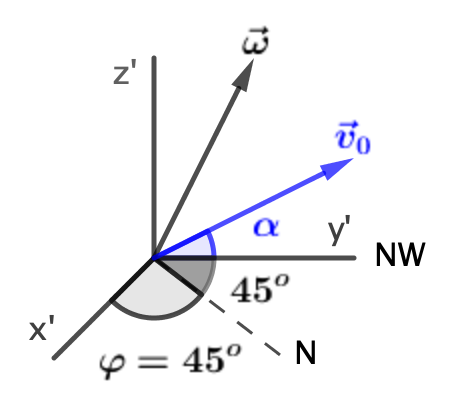
\includegraphics[width=.5\textwidth]{imagenes/imagenes10/T10IM17.png}
\end{figure}
\end{multicols}



\newpage %****************************************

\begin{myblock}{Experimento de Foucault}

\vspace{2mm} La primera exposición pública del péndulo de Foucault tuvo lugar en febrero de 1851, en el meridiano del Observatorio de París. Unas semanas más tarde, el físico francés Léon Foucault hizo su demostración más famosa en el interior del Panteón de París, cuando hizo suspender un péndulo de plomo de una masa de $28$ kg (una bala de cañón recubierta de latón) mediante un cable de $67$ metros de largo que pendía justo debajo del centro de la cúpula del Panteón. El plano de oscilación del péndulo giraba hacia la derecha $11^o$ por hora, haciendo un círculo completo en $32.7$ horas. El montaje original utilizado en 1851 en el Panteón fue trasladado en 1855 al Museo de Artes y Oficios de París. Una segunda instalación temporal se hizo en el Panteón, en 1902, para el 50 aniversario del experimento original.

\begin{figure}[H]
	\centering
	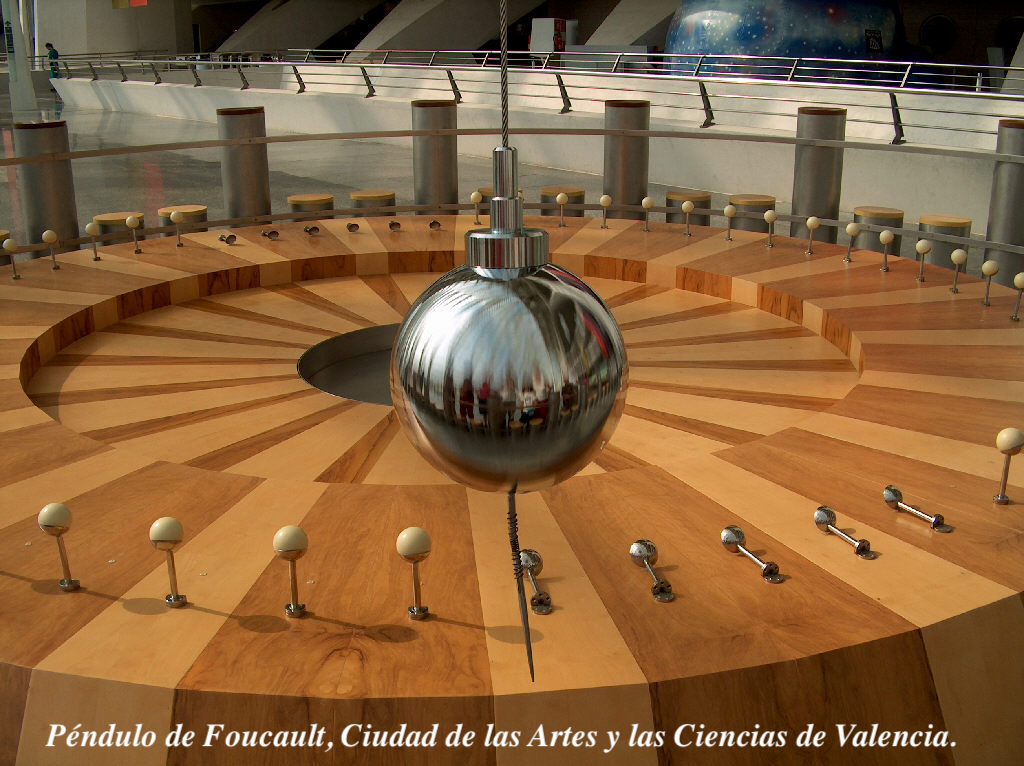
\includegraphics[width=.9\textwidth]{imagenes/imagenes11/T11IM12.png}
\end{figure}

\vspace{2mm} Durante la reconstrucción del museo en la década de 1990, el péndulo original se mostró temporalmente en el Panteón (1995), pero fue devuelto posteriormente al Museo de Artes y Oficios de París antes de su reapertura en 2000. El 6 de abril de 2010, el cable de suspensión del péndulo se rompió, causando daños irreparables en el péndulo y en el suelo de mármol del museo. Una copia exacta del péndulo original había estado oscilando de forma permanente desde 1995 bajo la cúpula del Panteón de París hasta 2014, cuando fue desmontado durante los trabajos de reparación en el edificio. En septiembre de 2017 el péndulo volvió a estar instalado y funcionando de nuevo.

\vspace{2mm} Hay muchos péndulos de Foucault exhibidos por el mundo, en Valencia en el Museo de las Ciencias Príncipe Felipe de la Ciudad de las Artes y las Ciencias existe otro péndulo de Foucault expuesto al público.	
\end{myblock}







